\documentclass[a4paper,fleqn]{cas-dc}
\usepackage[numbers,sort&compress]{natbib}
\usepackage{microtype}
\usepackage{placeins}
\usepackage{needspace}
\usepackage{xurl}
\usepackage[nospread]{flushend}
\hypersetup{hidelinks}
\setlength{\emergencystretch}{1em}
\setlength{\textfloatsep}{10pt plus 2pt minus 2pt}
\setlength{\floatsep}{8pt plus 2pt minus 2pt}
\setlength{\intextsep}{10pt plus 2pt minus 2pt}
\setlength{\dbltextfloatsep}{10pt plus 2pt minus 2pt}
\setlength{\dblfloatsep}{8pt plus 2pt minus 2pt}
\renewcommand{\floatpagefraction}{0.75}
\renewcommand{\dblfloatpagefraction}{0.75}
\makeatletter
\def\@dbflt#1{%
  \@ifnextchar[{\@xdblfloat{#1}}{%
    \edef\reserved@a{\noexpand\@xdblfloat{#1}[\csname fps@#1\endcsname]}%
    \reserved@a}}
\makeatother
\graphicspath{{figures/}}
\newcommand{\model}{MCGI-YOLO\xspace}
\newcolumntype{P}[1]{>{\raggedright\arraybackslash}p{#1}}

\begin{document}
\let\WriteBookmarks\relax
\let\printorcid\relax
\shorttitle{MCGI-YOLO for circular knitting}
\shortauthors{K. Tan et al.}

\title[mode=title]{A Defect Detection and Closed-Loop Control System with MCGI-YOLO for Circular Knitting Machines}

\author[1]{Kangzhao Tan}
\ead{tankangzhao@mails.gdut.edu.cn}

\author[1]{Jiarui Zhang}
\ead{zhangjiarui1@mails.gdut.edu.cn}

\author[1]{Junjie Yu}
\ead{yujunjie2@mails.gdut.edu.cn}

\author[2]{Heng Wu}
\ead{heng.wu@gdut.edu.cn}

\author[3]{Jing Lin}
\cormark[1]
\ead{lj@gdut.edu.cn}

\author[4]{Diyu Li}
\cormark[1]
\ead{lidiyu@vinsome.cn}

\author[1]{Chunhua He}
\cormark[1]
\ead{hechunhua@pku.edu.cn}

\affiliation[1]{organization={School of Computer Science, Guangdong University of Technology},
 city={Guangzhou}, postcode={510006}, country={China}}
\affiliation[2]{organization={School of Automation, Guangdong University of Technology},
 city={Guangzhou}, postcode={510006}, country={China}}
\affiliation[3]{organization={Classroom Management Center, Guangdong University of Technology},
 city={Guangzhou}, postcode={510006}, country={China}}
\affiliation[4]{organization={Guangzhou Vinsome Automation Technology Co., Ltd.},
 city={Guangzhou}, country={China}}
\cortext[1]{Corresponding authors: Jing Lin, Diyu Li, and Chunhua He.}

\begin{abstract}
Fabric inspection after knitting can identify defective cloth, but the material loss has already occurred when persistent yarn or needle abnormalities are discovered. This paper presents an inspection workflow that integrates defect detection and intervention into circular knitting. A dedicated system combines rotation-activated detection, continuous image acquisition, controlled illumination, coaxial image transmission, edge inference, configurable machine stopping, and cloud notification. It continuously inspects fabric during formation and stops production when detected defects exceed the selected acceptance criteria, limiting further defective fabric production and reducing dependence on sustained human visual attention. To support this workflow on a resource-constrained edge device, we develop \model. Morphology-aware context encoding (MCE) captures the spatial continuity of horizontal and vertical elongated defects, while gated interpolation upsampling (GIU) adapts feature reconstruction to different defect morphologies and scales. On a production-line dataset, \model achieves 97.2\% mAP@50 and 65.5\% mAP@50:95, exceeding YOLOv8n by 6.7 and 7.1 percentage points. After INT8 conversion, it achieves 96.7\% mAP@50 and 64.0\% mAP@50:95 at 23 FPS on the edge device. At a collaborating factory operating 48 circular knitting machines, factory-provided estimates indicate a reduction in average monthly fabric waste from 2030 to 148 kg. The results connect accurate edge detection with a change in inspection organization and reduced material loss during production.
\end{abstract}
\begin{keywords}
Circular knitting machine \sep Edge computing \sep Fabric defect detection \sep Gated interpolation upsampling \sep Morphology-aware context encoding \sep YOLO
\end{keywords}
\maketitle

\section{Introduction}
Circular knitting machines are key production equipment for high-volume weft-knit fabric, which is widely used in everyday clothing such as T-shirts and sportswear \cite{cottonworksKnitBasics,woolmarkCircularKnitting,cottonworksSingleDouble}. The International Textile Manufacturers Federation reported approximately 24,500 global shipments of circular knitting machines in 2025 \cite{itmf2025press}. Globally, approximately 92 million tonnes of textile waste are generated annually, highlighting the importance of reducing avoidable material losses \cite{unep2025textilewaste}. Conventional quality checks are often performed after knitting is completed. A persistent needle or yarn abnormality can therefore generate repeated defects along the fabric before discovery, accumulating substantial fabric waste and economic losses \cite{takeuchi2018knitted,akter2022material,xiang2023hooknet}. To prevent such losses, real-time detection during knitting is needed to identify these defects early and enable timely intervention before further defective fabric is produced.

Conventional fabric inspection typically separates production from quality control: completed fabric rolls are transferred to dedicated inspection machines, where operators examine the moving cloth under illumination, as illustrated in Fig.~\ref{fig:traditional-inspection} \cite{kumar2008survey}. This manual inspection workflow has several limitations. First, prolonged visual inspection easily causes operator fatigue, increasing the risk of missed defects. Second, human judgment is inherently subjective, making it difficult to establish consistent inspection standards and leading to both missed detections and false alarms \cite{xu2025zdm}. Third, manual inspection is relatively inefficient and struggles to keep pace with high-speed knitting production.

\begin{figure*}[width=\textwidth,pos=!tbp]
\centering
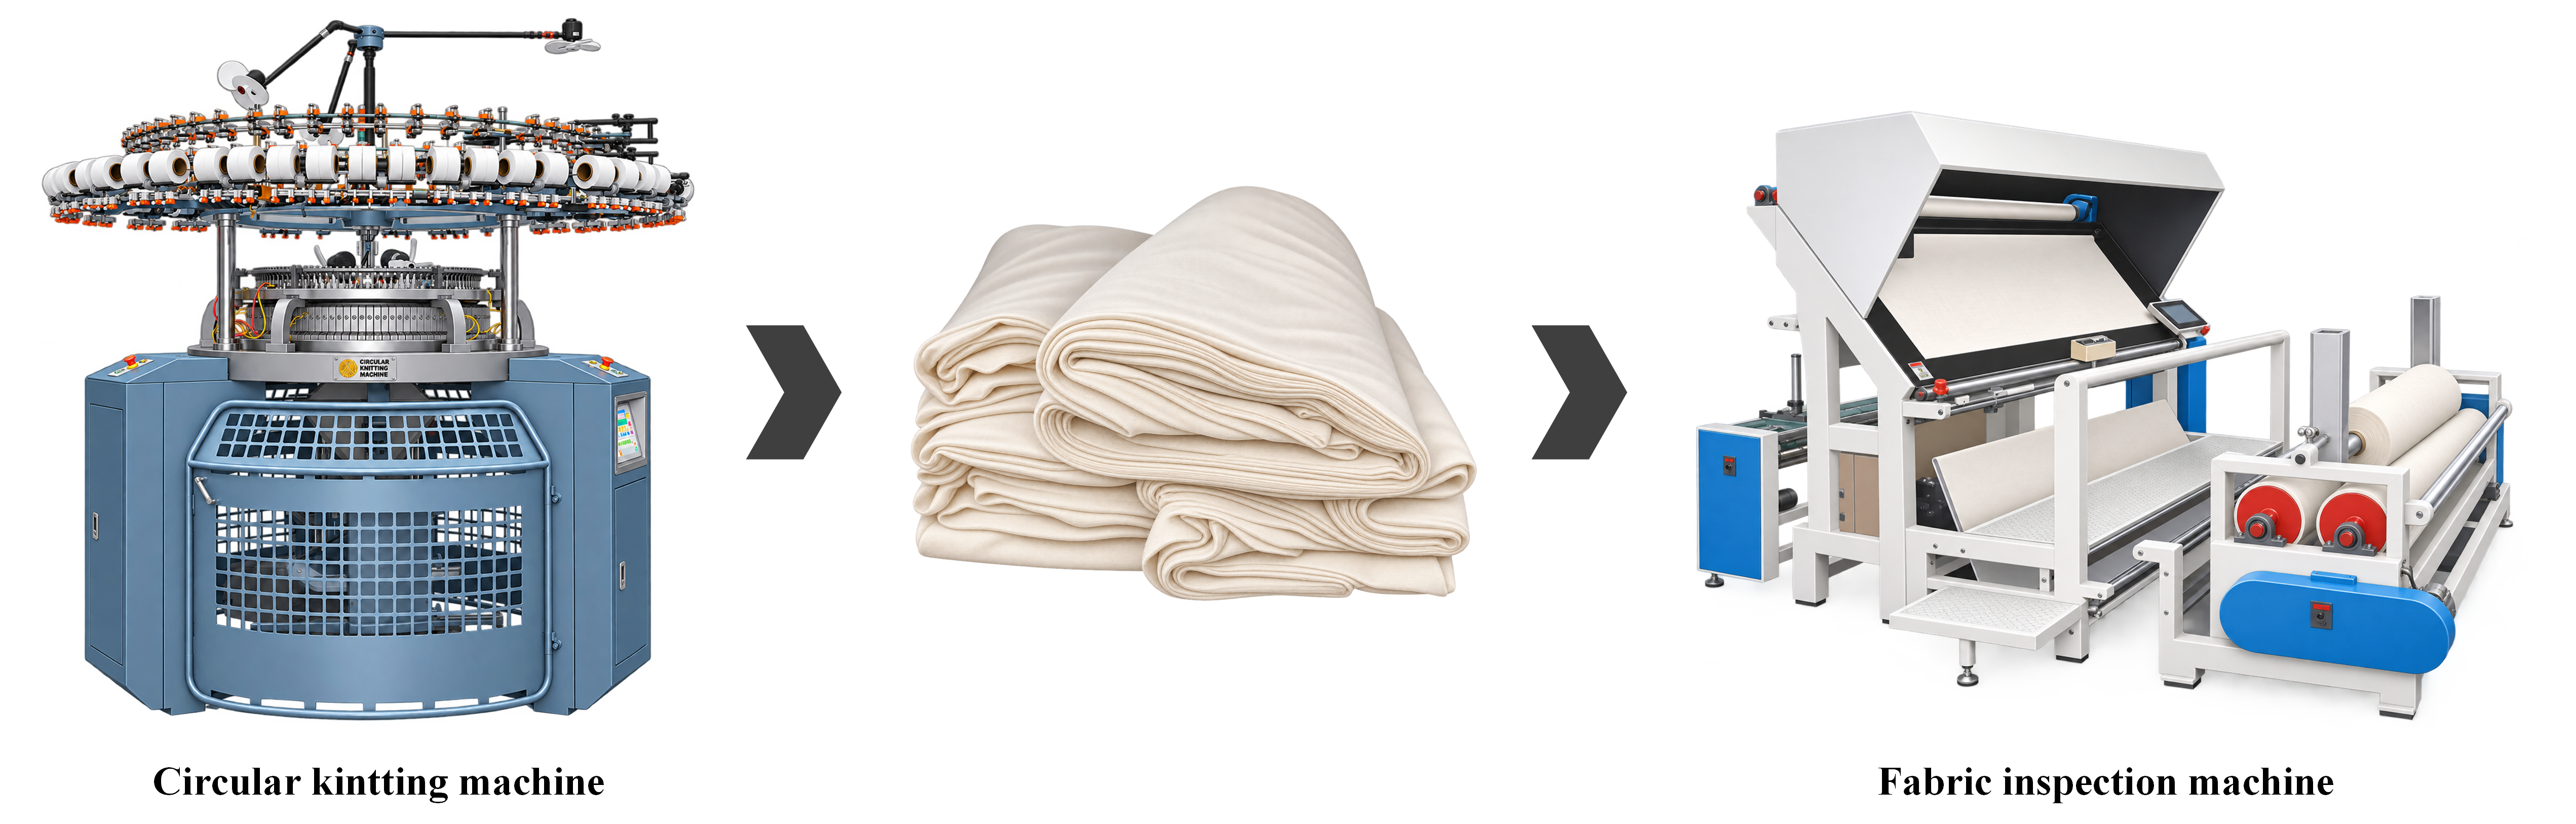
\includegraphics[width=\textwidth]{inspection.png}
\caption{Conventional post-production fabric inspection workflow.}
\label{fig:traditional-inspection}
\end{figure*}

To address these issues, machine-vision-based fabric inspection systems have been proposed, in which cameras and processing units are installed on inspection machines to replace human observation \cite{kumar2008survey,machado2025edgefabric}. Although such systems mitigate the drawbacks of manual inspection, they still operate as post-production inspection: defects are identified only after the fabric has been produced, by which time substantial defective material may already have accumulated, resulting in economic loss. Therefore, real-time inspection during the knitting process, coupled with closed-loop machine control, is needed to detect developing defects and trigger timely intervention.

To this end, we have developed a complete defect detection and closed-loop control system embedded directly into circular-knitting production. At the hardware level, the system integrates a global-shutter camera, LED illumination, coaxial SerDes transmission, a Hall sensor for rotation-activated detection, and an edge computing device, together with interfaces for local machine stopping and remote monitoring. At the algorithmic level, guided by systematic observations of defect morphologies arising during the knitting process, we develop a lightweight fabric defect detector based on YOLOv8n \cite{ultralytics2023}. The detector incorporates a morphology-aware context encoding (MCE) module to capture the extended spatial continuity of horizontal and vertical elongated defects, and a gated interpolation upsampling (GIU) module to enable content-adaptive feature reconstruction for defects of diverse shapes and scales, all under the stringent computational budget of edge deployment. To translate detection results into stopping decisions, we introduce a user-configurable post-NMS stopping module. It combines confidence, class-specific geometric thresholds, and per-frame defect counts to accommodate different factory quality requirements and trigger local machine stopping when the configured criteria are met.

The main contributions are as follows.
\begin{enumerate}
  \renewcommand{\labelenumi}{\arabic{enumi})}
  \item We develop an embedded defect detection and closed-loop control system for circular-knitting production, integrating rotation-activated detection, continuous image acquisition, illumination, SerDes transmission, edge processing, and machine-control interfaces.
  \item We propose \model, a lightweight detector incorporating MCE and GIU to address elongated-defect continuity and multiscale feature reconstruction under edge-computing constraints. A user-configurable post-NMS stopping module further translates detection outputs into local machine-stop decisions according to factory quality requirements.
  \item We deploy the system in a textile factory, where it enables inspection and intervention during knitting and reduces fabric waste, demonstrating its practical production value.
\end{enumerate}

The remainder of this paper is organized as follows. Section~\ref{sec:related-work} reviews inspection workflows, edge systems, and detection algorithms. Section~\ref{sec:system-design} presents the system design, and Section~\ref{sec:method} describes the detection method. Section~\ref{sec:results} reports the experimental protocol and results. Section~\ref{sec:system-operation} presents deployment, system operation, and industrial application. Section~\ref{sec:conclusion} concludes the paper.

\section{Related Work}
\label{sec:related-work}
\subsection{Fabric Inspection Systems}
Offline fabric inspection examines produced fabric on inspection or winding machines by integrating image acquisition, illumination, and defect recognition. Barman et al. installed a Haar-wavelet processing and random-forest classification system on a fabric inspection machine operating at 30 m/min \cite{barman2022inspectionmachine}, and Kuo et al. combined a CMOS camera, front and back illumination, and SVM classification to detect eight woven-fabric defect types on a winding machine at 20 m/min \cite{kuo2022woveninspection}. More recent systems apply deep learning to offline fabric inspection. Machado et al. installed cameras above a fabric rolling line and deployed YOLO11n on a Jetson Orin Nano to inspect solid-color cotton and linen fabrics \cite{machado2025edgefabric}. Zhao et al. deployed an edge--cloud collaborative system on a fabric inspection machine, with real-time detection at the edge and cloud-based data management and algorithm adaptation through transfer learning \cite{zhao2020edgecloud}.

Although offline fabric inspection improves inspection efficiency, defects arising during knitting may continue to accumulate before they are identified. On-machine defect detection brings recognition closer to fabric formation and enables earlier intervention. Saeidi et al. implemented Gabor-wavelet analysis and neural-network classification on a circular knitting machine \cite{saeidi2005vision}. \c{C}elik et al. combined image acquisition, illumination, encoder-based synchronization, and CNN-based classification for on-machine defect detection during circular knitting \cite{celik2022circular}. These studies demonstrate the feasibility of this approach. Scaling it across multiple knitting machines requires consideration of per-machine camera and processor costs, the computational resources needed for continuous inference, and integration with machine-control interfaces. Camera and processor selection must therefore be considered together with the recognition method and the required inspection throughput.

\subsection{Fabric Defect Detection Algorithms}
Fabric defect detection requires distinguishing local abnormalities from regular, directionally structured fabric textures. Early methods relied on handcrafted features derived from statistical analysis, spectral transforms, or analytical models \cite{kumar2008survey,ngan2011review}. Although effective under relatively controlled conditions, these methods often depend on predefined texture representations, limiting their adaptability to variations in fabric patterns and defect morphology. Deep learning-based detectors overcome some of these limitations through learned feature representations. Among them, YOLO-based methods combine defect localization with efficient inference, making them suitable candidates for on-machine defect detection \cite{redmon2016yolo}.

Recent studies have improved detection performance through enhanced feature extraction and multiscale fusion. FA-YOLO combines receptive-field enhancement, attention, and adaptive spatial feature fusion \cite{yu2024fayolo}, while DGHR-YOLO introduces deformable convolution and a high-level screening feature pyramid \cite{zhang2025dghr}. Attention-based multiscale feature fusion enhances weak defect responses through intralayer enhancement and cross-layer interaction \cite{zhao2024amff}. JDCBL combines contextual Transformer features with balanced contrastive learning to address scale variation and long-tailed defect categories \cite{an2025jdcbl}. For elongated and tilted fabric defects, RRNet employs position-guided fusion and multiscale rotation-guided strip coupling \cite{wang2026rrnet}. Although these methods improve feature representation and detection performance, incorporating attention mechanisms, deformable convolutions, Transformers, and complex multiscale fusion can introduce additional computational and memory overhead. Such overhead is particularly relevant to continuous defect detection on resource-constrained edge processors. Therefore, effective on-machine detection requires balancing morphology-aware feature extraction, multiscale feature reconstruction, and computational efficiency to support practical industrial deployment.

\section{System Design}
\label{sec:system-design}
\subsection{System Overview}
\label{sec:system-overview}
\begin{figure*}[width=\textwidth,pos=!tbp]
\centering
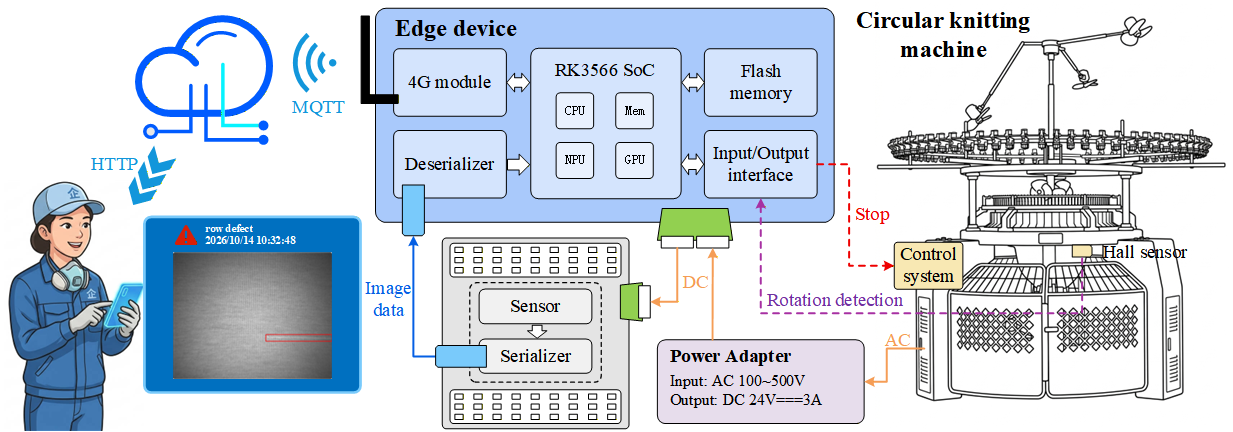
\includegraphics[width=1.0\textwidth]{fig1.png}
\caption{Overview of the proposed defect detection and closed-loop control system.}
\label{fig:interactions}
\end{figure*}

We design and implement a dedicated defect detection and closed-loop control system for circular knitting machines, as shown in Fig.~\ref{fig:interactions}. The closed-loop workflow begins when the operator starts the machine. The Hall sensor detects machine rotation and triggers the edge device to activate the camera and LED illumination for continuous image acquisition and defect detection. When a detected defect satisfies the configured stopping criteria, the edge device immediately sends a stop command to the machine controller to prevent further defect propagation, uploads the defect image and record to the cloud, and pushes an alert notification to the operator. After the operator inspects the reported defect, resolves the production fault, and restarts the machine, the rotation signal reactivates detection. This sequence forms a complete production–detection–control loop. The system is organized into three functional subsystems: power supply, image acquisition and transmission, and processor. The following subsections describe their designs and hardware implementation.

\subsection{Power Supply Subsystem}
To accommodate different industrial supply voltages across countries and regions, we design a power adapter with a 100--500 V AC input range and a 24 V DC output rated at 3 A. The adapter first supplies this output to the device. The device then supplies the LED illumination. By adjusting the current delivered to the LEDs, the device controls the illumination brightness to suit the image-acquisition conditions. This arrangement integrates LED power delivery and brightness control into the device.

\subsection{Image Acquisition and Transmission Subsystem}
The rapid rotation of circular knitting machines requires imaging that preserves defect geometry and fine spatial detail. We therefore select a SmartSens SC130GS global-shutter sensor (SmartSens Technology Co., Ltd., Shanghai, China) at $1280\times1024$ resolution, which exposes all pixels simultaneously to avoid motion-induced distortion from sequential row exposure. At a camera-to-fabric distance of approximately 10 cm, the field of view is approximately $16\times12$ cm, with the 16 cm horizontal width $w$ aligned with the direction of fabric motion.

Cost is also a practical constraint when equipping multiple knitting machines; Table~\ref{tab:camera-costs} compares the selected camera assembly with camera configurations used in previous fabric-inspection systems.

\begin{table}[pos=!htbp]
\caption{Camera configurations and reference costs.}
\label{tab:camera-costs}
\centering
\footnotesize
\setlength{\tabcolsep}{3pt}
\renewcommand{\arraystretch}{1.1}
\begin{tabular}{@{}P{0.23\columnwidth}P{0.48\columnwidth}P{\dimexpr0.29\columnwidth-12pt\relax}@{}}
\toprule
Study & Hardware & Cost (USD) \\
\midrule
Kuo et al.\cite{kuo2022woveninspection} & Basler acA4600-10uc & 739 \\
\c{C}elik et al.\cite{celik2022circular} & Basler raL2048-48gm & 1309 \\
Machado et al.\cite{machado2025edgefabric} & $2\times$Intel RealSense D435i & 399/unit \\
Zhao et al.\cite{zhao2020edgecloud} & Line-scan CCD & $\approx1400^{\dagger}$ \\
Ours & SC130GS camera with serializer & $\approx52$ \\
\bottomrule
\end{tabular}
\par\smallskip
\begin{minipage}{\columnwidth}
\footnotesize
$\dagger$The original study does not report the camera model; the reference price is approximately USD 1400.
\end{minipage}
\end{table}

Factory machinery creates an electromagnetically noisy environment, and installation requires the camera and edge device to be separated by a cable run. We therefore use serializer/deserializer (SerDes) transmission over shielded coaxial cable to accommodate remote camera placement and the interference environment. Specifically, the THCV241A serializer and THCV242A deserializer (THine Electronics, Inc., Tokyo, Japan) bridge the camera-side and processor-side MIPI CSI-2 interfaces. As illustrated in Fig.~\ref{fig:serdes}, the serializer converts the camera output into a serial stream, which is transmitted over the coaxial cable and recovered by the deserializer for the RK3566. Power over Coax (PoC) supplies the camera side through the same cable, combining image transmission and power delivery in a single connection. The link supports a maximum serial line rate of 4.0 Gb/s per lane, corresponding to a rated effective rate of 3.2 Gb/s \cite{thineTHCV241A,thineTHCV242A}.

\begin{figure}[pos=!htbp]
\centering
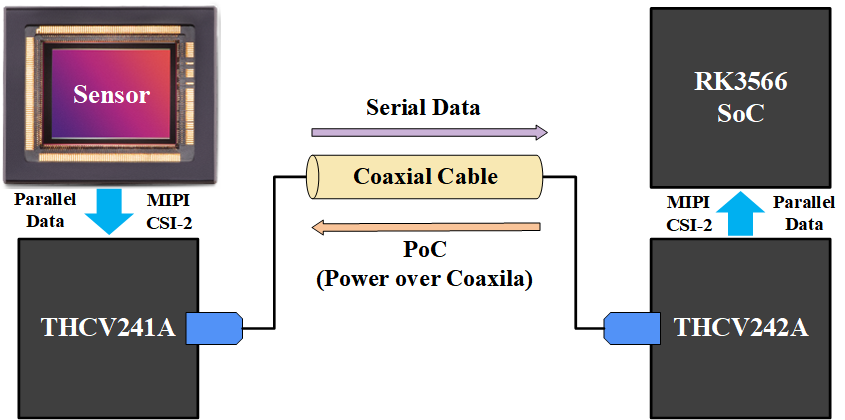
\includegraphics[width=\columnwidth]{serdes.png}
\caption{SerDes image-transmission link with coaxial power delivery.}
\label{fig:serdes}
\end{figure}

The camera is configured to transmit $1280\times1024$ RAW10 images at 30 frames/s. With $b=10$ bits per pixel, the active-image payload rate is
\begin{equation}
\begin{aligned}
R_{\mathrm{img}} &= W H b f_{\mathrm{cam}} \\
&=1280\times1024\times10\times30 \\
&=393.216\ \mathrm{Mb/s},
\end{aligned}
\label{eq:serdes-bandwidth}
\end{equation}
\noindent where $W$ and $H$ denote the image width and height, and $f_{\mathrm{cam}}$ is the camera acquisition rate. This corresponds to only 12.3\% of the rated single-lane effective capacity, providing a stable image input for the detection system.

\subsection{Processor Subsystem}
\label{sec:coverage}
We derive the processor-throughput target from the production conditions in Table~\ref{tab:production-inputs} and the camera field of view before selecting the hardware.

\begin{table}[pos=!htbp]
\caption{Machine operating parameters.}
\label{tab:production-inputs}
\centering
\footnotesize
\setlength{\tabcolsep}{3pt}
\renewcommand{\arraystretch}{1.08}
\begin{tabular*}{\columnwidth}{@{\extracolsep{\fill}}llr@{}}
\toprule
Parameter & Symbol & Value \\
\midrule
Design machine diameter & $D$ & 1.016 m (40 in) \\
Rotation period & $T$ & 2 s/revolution \\
\bottomrule
\end{tabular*}
\end{table}

With fabric moving at $\pi D/T$ and a horizontal field-of-view width of $w=0.16$ m, the minimum coverage rate is
\begin{equation}
f_{\min}=\frac{\pi D}{Tw}
=\frac{\pi\times1.016}{2\times0.16}
\approx9.97\ \mathrm{frames/s},
\label{eq:coverage-rate}
\end{equation}
\noindent establishing 10 frames/s as the throughput target for hardware selection. Rockchip's official RKNN Model Zoo reports a model-inference throughput of 35.1 FPS for INT8 YOLOv8n with $640\times640$ inputs in its RK3566/RK3568 benchmark, measured at the maximum NPU frequency \cite{rockchipmodelzoo}. This reference throughput is more than three times the 10 FPS requirement, providing an initial performance margin for task-specific algorithm improvements. We therefore select YOLOv8n as the baseline detector and the Rockchip RK3566 (Rockchip Electronics Co., Ltd., Fuzhou, China) as the processor, considering this margin, camera connectivity, and hardware cost (Table~\ref{tab:processor-costs}). The RK3566 integrates a quad-core Cortex-A55 CPU and an NPU rated at 1 TOPS for INT8 operations \cite{rockchiprk3566}.

\begin{table}[pos=!htbp]
\caption{Computing platforms and reference costs.}
\label{tab:processor-costs}
\centering
\footnotesize
\setlength{\tabcolsep}{3pt}
\renewcommand{\arraystretch}{1.1}
\begin{tabular}{@{}P{0.23\columnwidth}P{0.48\columnwidth}P{\dimexpr0.29\columnwidth-12pt\relax}@{}}
\toprule
Study & Hardware & Cost (USD) \\
\midrule
\c{C}elik et al.\cite{celik2022circular} & Desktop computer (unspecified) & $\approx1200^{\dagger}$ \\
Machado et al.\cite{machado2025edgefabric} & Jetson Orin Nano & $399^{\ddagger}$ \\
Ours & RK3566 board with deserializer & $\approx75$ \\
\bottomrule
\end{tabular}
\par\smallskip
\begin{minipage}{\columnwidth}
\footnotesize
$\dagger$Estimated cost of a general-purpose desktop. $\ddagger$Current Orin Nano Super Developer Kit reference price. Estimates and reference listings do not represent the studies' purchase costs.
\end{minipage}
\end{table}

\subsection{Network Communication Subsystem}
The edge device connects to the cloud through a 4G module with a SIM-card slot and an external antenna interface. This connection supports defect-image and event uploads, alert notifications, device-state reporting, and remote client configuration. The client and cloud functions are detailed in Section~\ref{sec:system-operation}.

\subsection{Hardware Implementation}
\label{sec:hardware-implementation}
Based on the design requirements of the subsystems described above, we develop the corresponding hardware shown in Fig.~\ref{fig:hardware}.

\begin{figure*}[width=\textwidth,pos=!tbp]
\centering
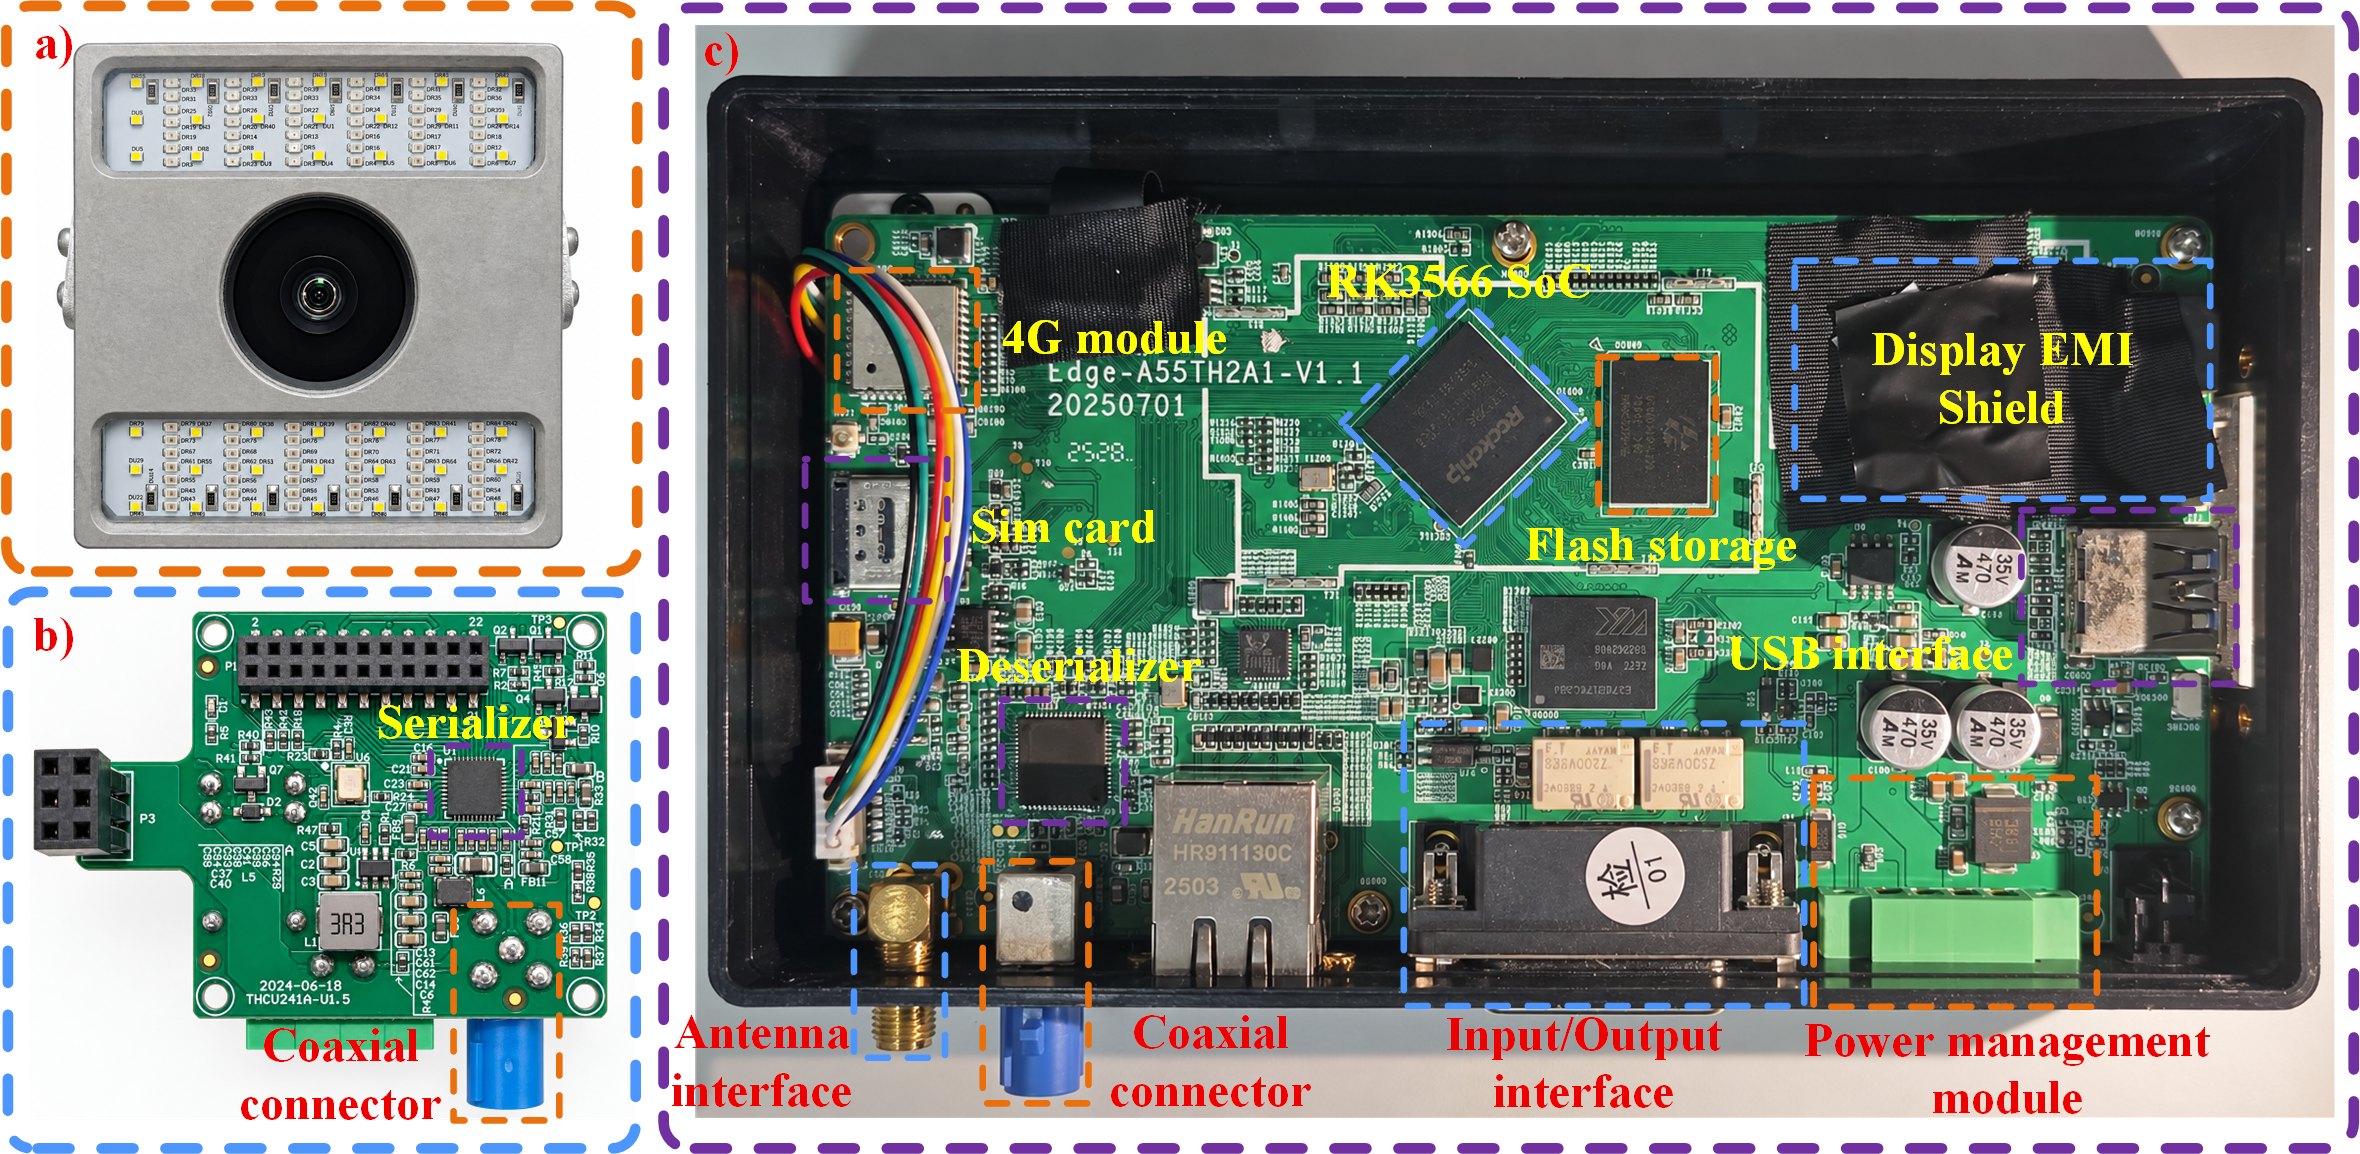
\includegraphics[width=1.0\textwidth]{fig2.png}
\caption{System hardware: (a) camera and illumination, (b) camera interface board, and (c) RK3566 edge board.}
\label{fig:hardware}
\end{figure*}

The camera assembly (a) combines the image sensor and LED illumination. We design a camera-side interface board (b) that integrates the serializer and coaxial connector, and a mainboard (c) built around the RK3566. The mainboard integrates flash storage, the camera deserializer and coaxial connector, a 4G module with SIM-card and antenna interface, input/output interface, and power-management circuitry. This board-level integration brings image reception, local inference, network communication, machine control, and illumination control into a dedicated edge device. Fig.~\ref{fig:system} shows the system installed on a circular knitting machine in a real production line.

\begin{figure*}[width=\textwidth,pos=!tbp]
\centering
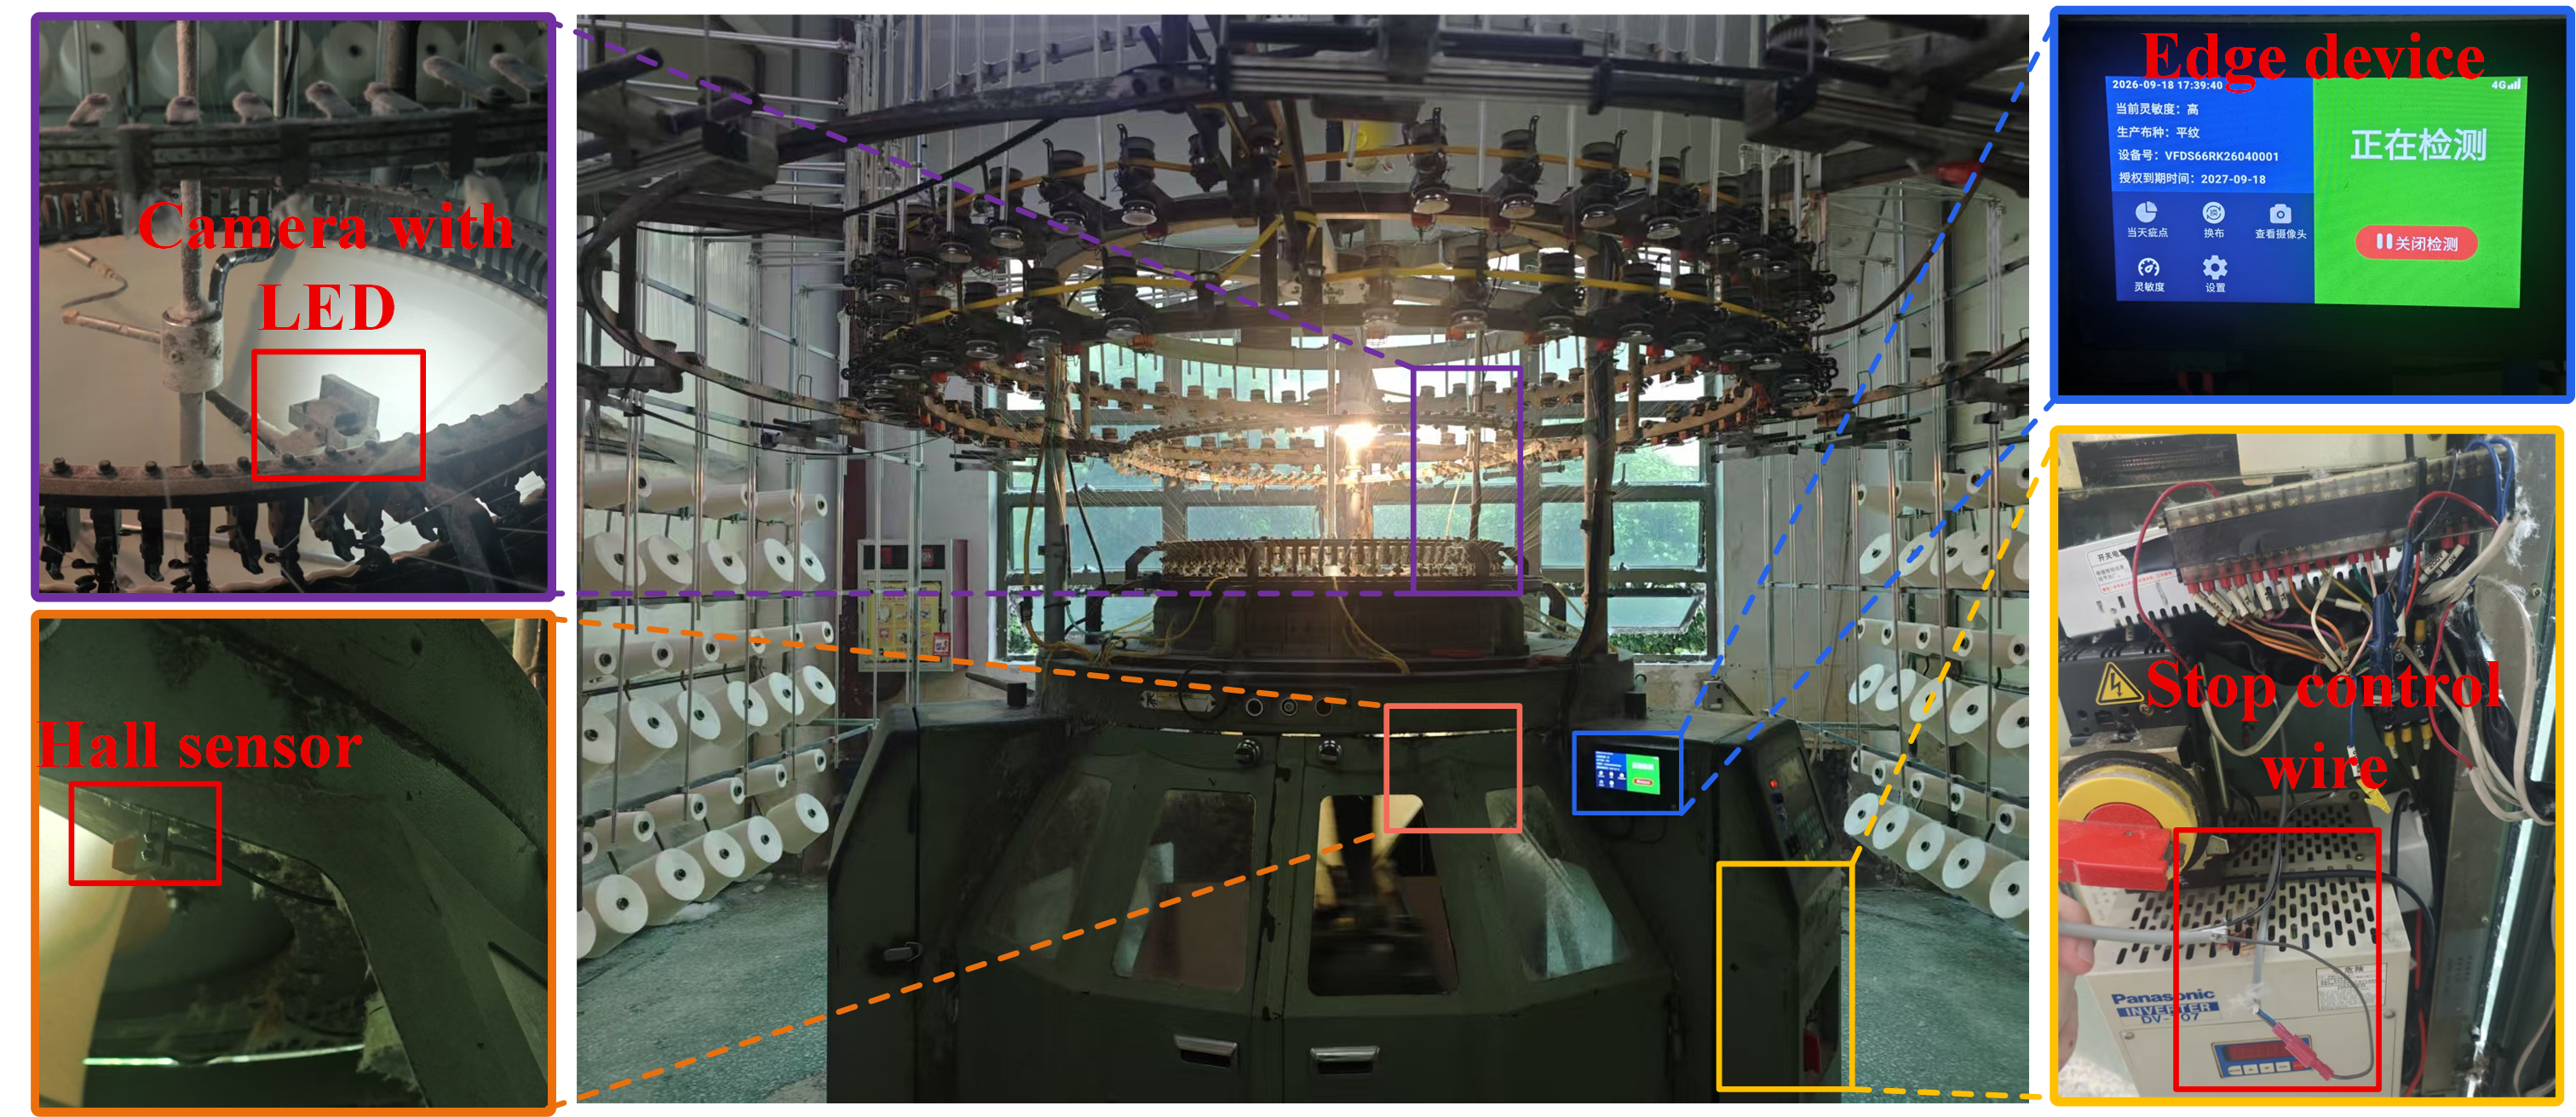
\includegraphics[width=1.0\textwidth]{fig3.png}
\caption{System installation on a circular knitting machine.}
\label{fig:system}
\end{figure*}

\section{Detection Method}
\label{sec:method}
\subsection{Defect Morphology and Design Motivation}
\label{sec:defect-morphology}
Fig.~\ref{fig:dataset-examples} presents typical defects encountered during circular knitting. Horizontal and vertical defects extend over long spatial ranges while remaining narrow in the perpendicular direction, and their visible lengths vary considerably. Holes range from small localized openings to large damaged regions, and different defect categories may coexist in the same image. These observations indicate that the detector must associate spatially separated responses along elongated defects while accommodating substantial differences in defect shape and scale.

\begin{figure*}[width=\textwidth,pos=!tb]
\centering
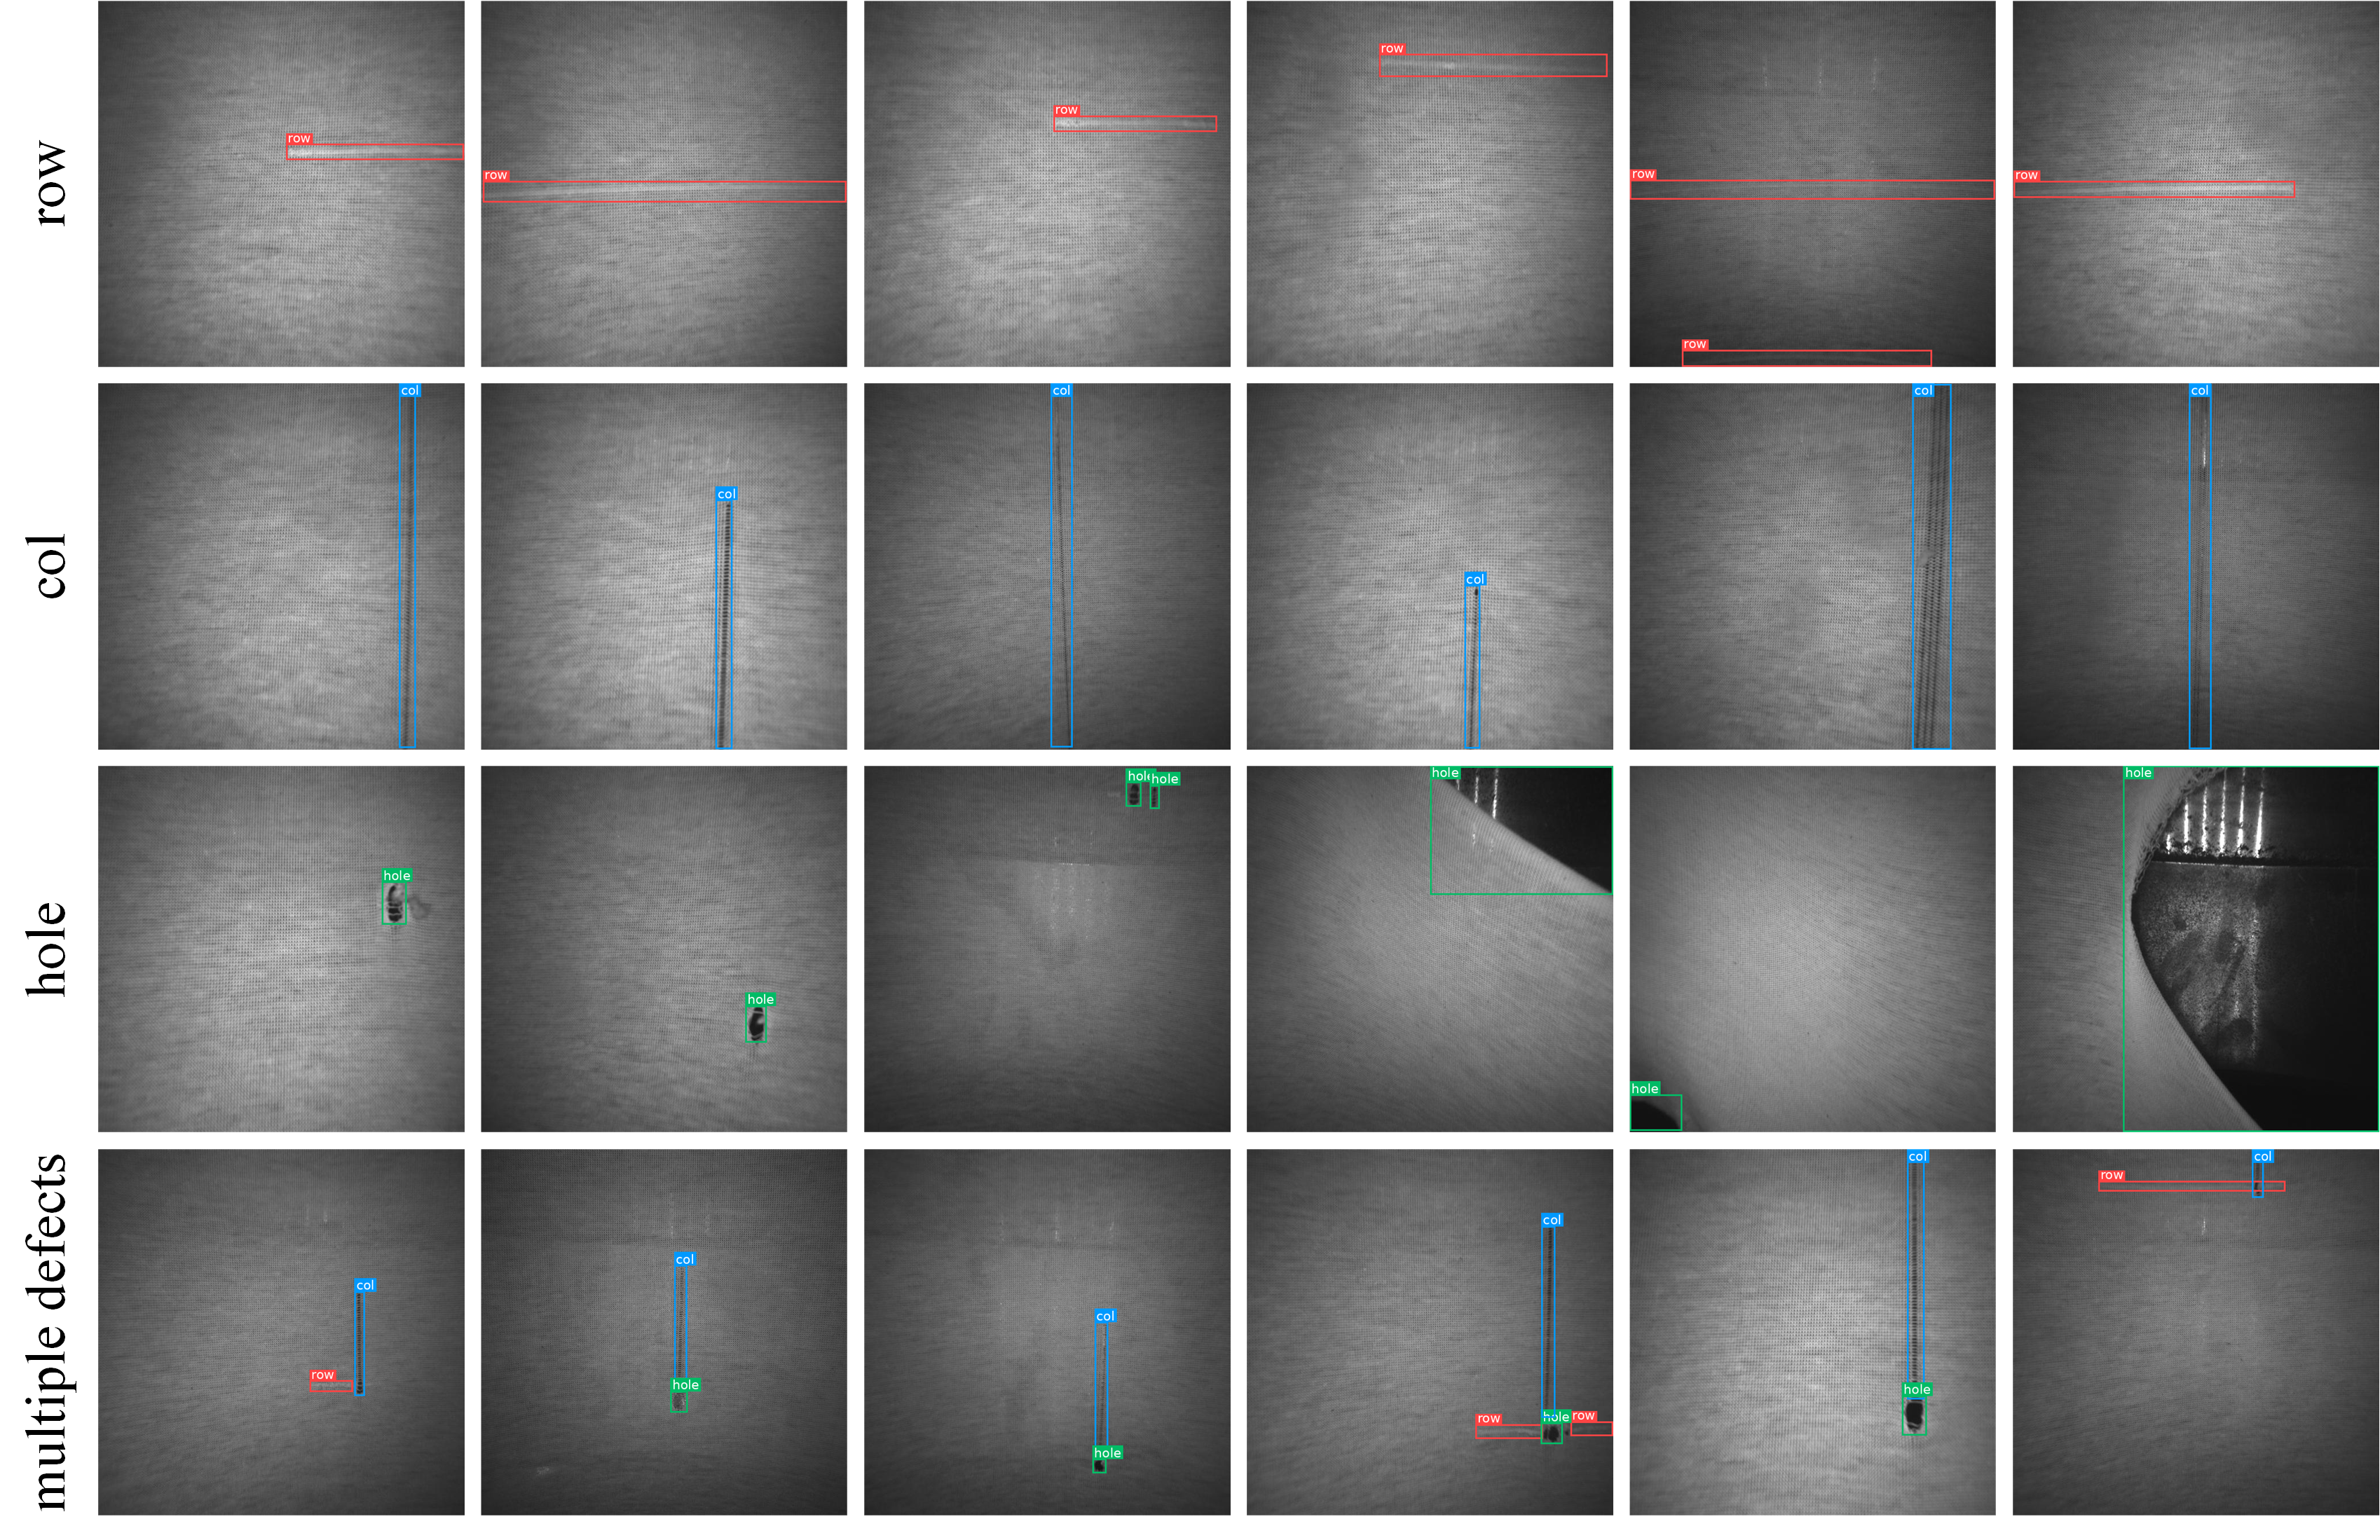
\includegraphics[width=\textwidth]{defect.png}
\caption{Representative annotated fabric-defect samples.}
\label{fig:dataset-examples}
\end{figure*}

Fig.~\ref{fig:annotation-shapes} summarizes the morphology and scale variation of the 468 annotated boxes. Each box is translated to the common center $(0.5,0.5)$ while retaining its width and height normalized by the image dimensions. Horizontal and vertical defects form distinct elongated distributions, whereas holes span a wide range of spatial extents. These distributions highlight two detection requirements: associating distant responses along elongated defects and preserving spatial structure across defects of different shapes and scales under the computational constraints of edge deployment.

\begin{figure*}[width=\textwidth,pos=!tb]
\centering
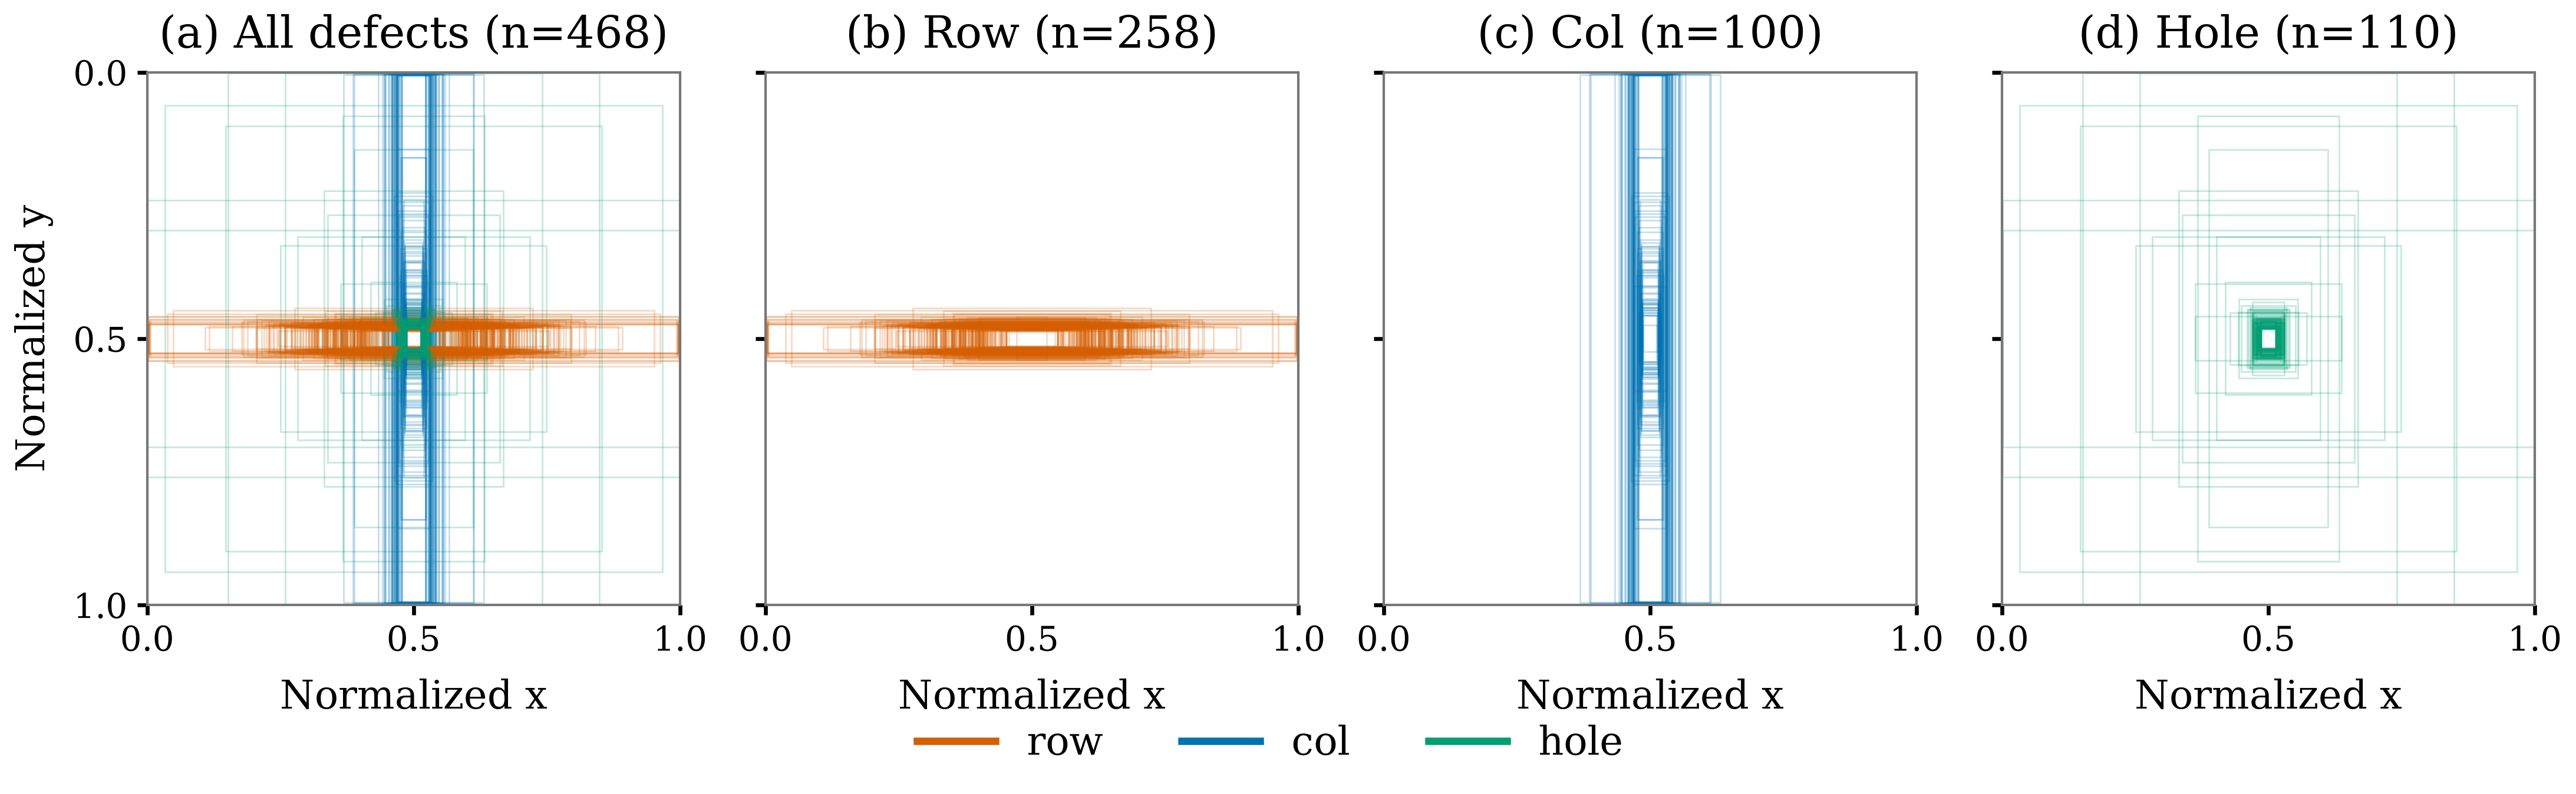
\includegraphics[width=\textwidth]{annotation_shapes.png}
\caption{Centered bounding-box distributions for all defects and each defect category.}
\label{fig:annotation-shapes}
\end{figure*}

\subsection{MCGI-YOLO Architecture}
Fig.~\ref{fig:network} shows \model based on YOLOv8n \cite{ultralytics2023}. To associate spatially separated responses along horizontal and vertical elongated defects, morphology-aware context encoding (MCE) is embedded in the P3 and P4 backbone C2f blocks. To accommodate differences in defect shape and scale during feature reconstruction, gated interpolation upsampling (GIU) replaces the two top-down upsampling operations from P5 to P4 and from P4 to P3, adapting higher-level context to local feature content before fusion with lateral features. The remaining backbone, bottom-up path, and detection head are retained \cite{lin2017fpn,liu2018panet}.

\begin{figure*}[width=\textwidth,pos=!tb]
\centering
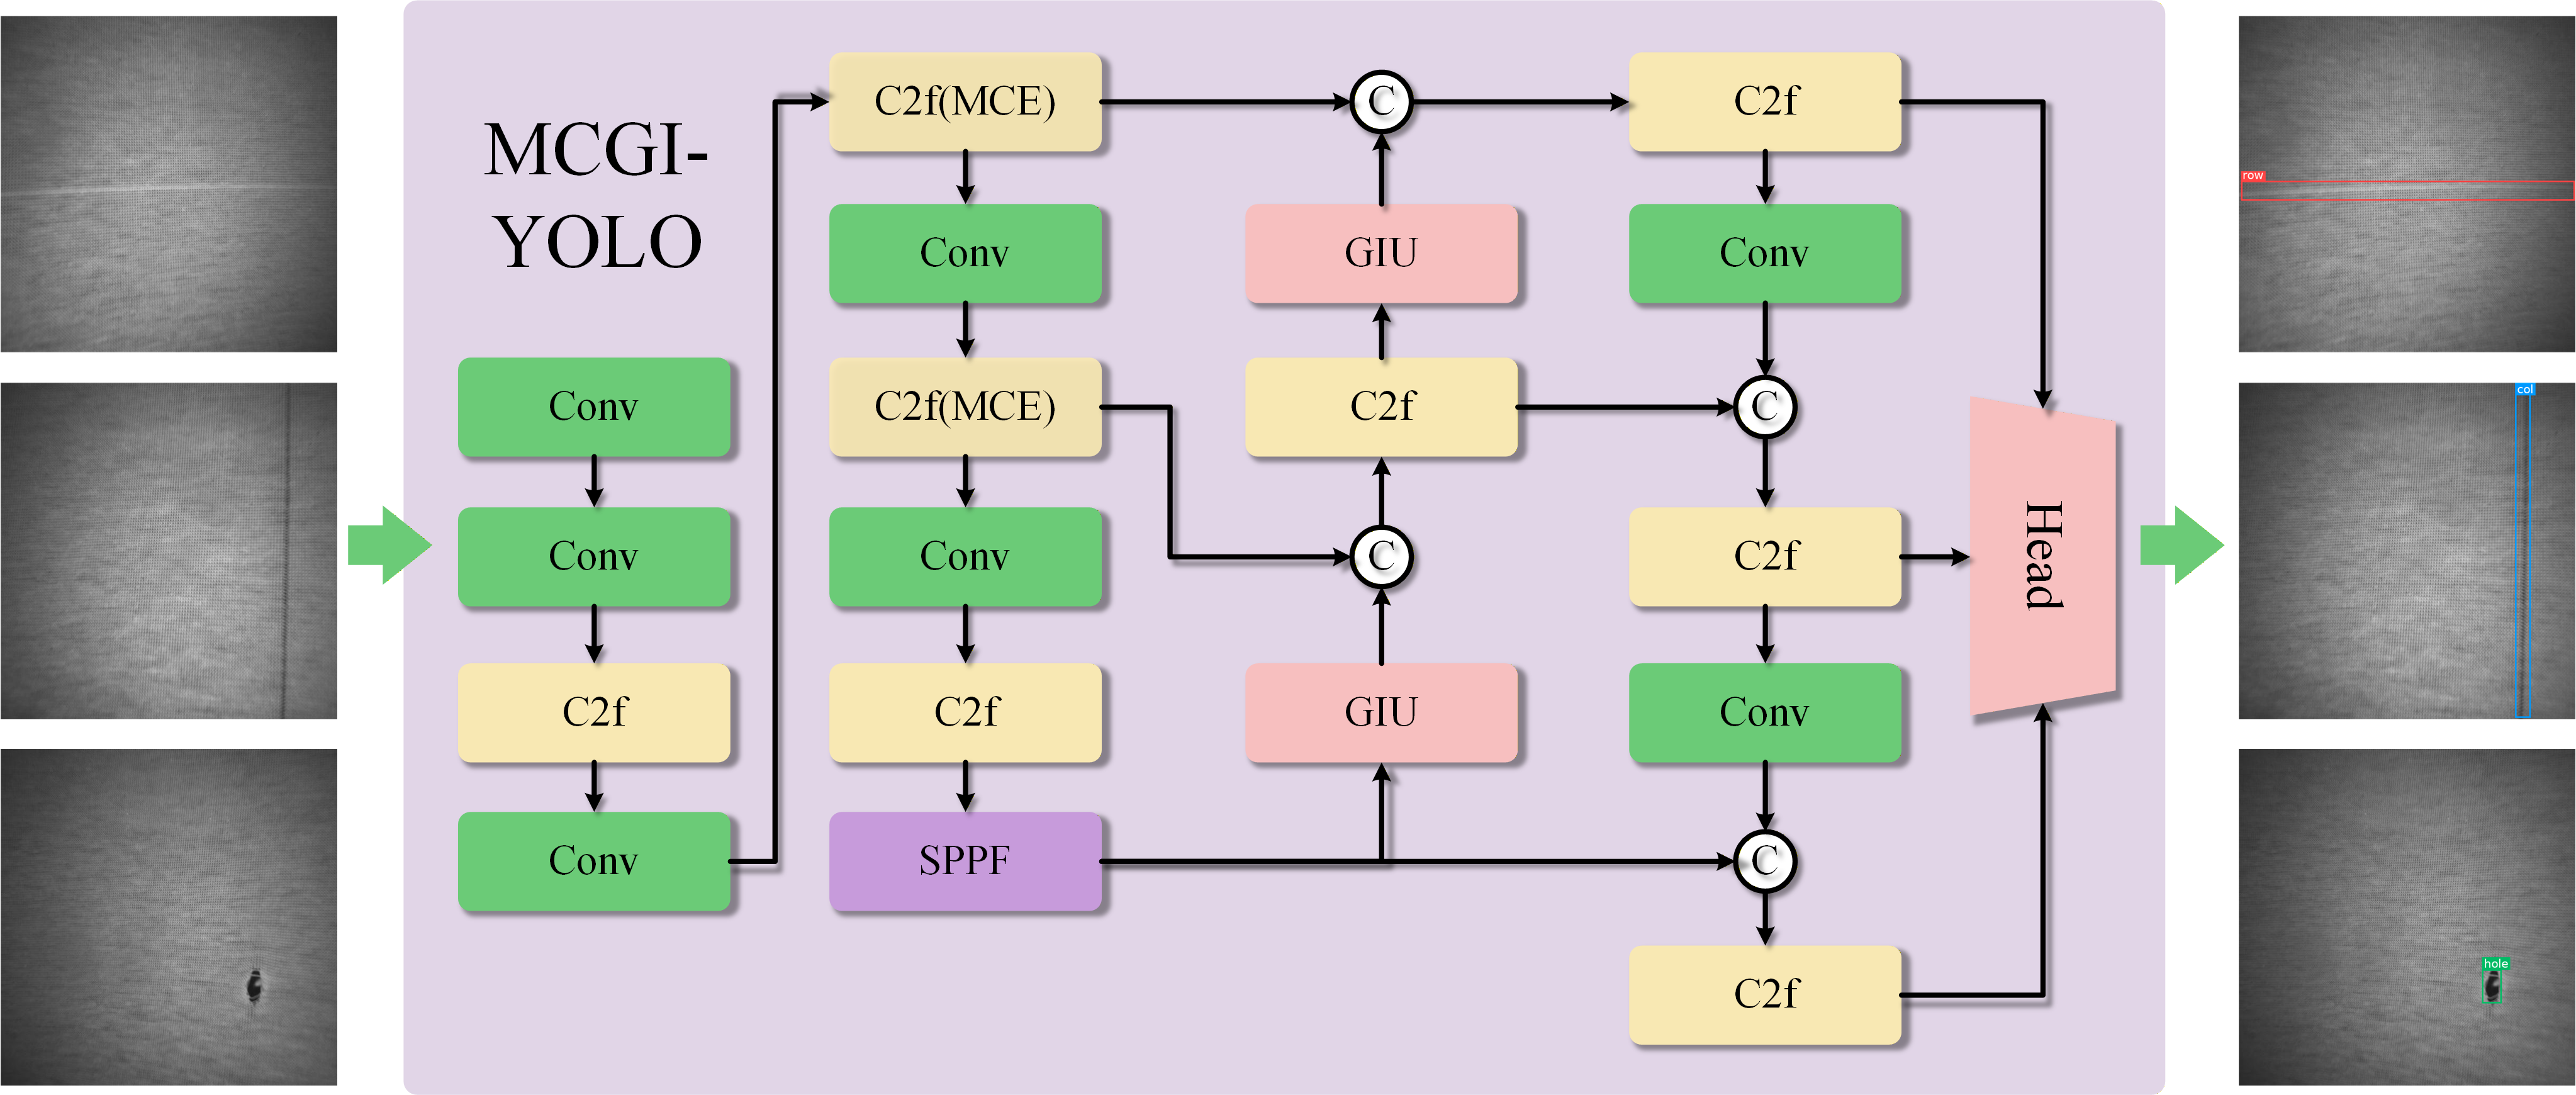
\includegraphics[width=0.9\textwidth]{fig4.png}
\caption{Architecture of \model.}
\label{fig:network}
\end{figure*}

\subsection{Morphology-Aware Context Encoding}
MCE focuses on horizontal and vertical elongated defects produced by circular knitting machines. Elongated defects are characterized by a high aspect ratio. Their continuity spans across large spatial regions, making it difficult for local receptive fields to establish long-range dependencies. Local feature extraction alone fails to explicitly associate these spatially separated responses as parts of the same defect. Meanwhile, modeling long-range dependencies through dense channel-wise interactions would introduce substantial redundancy, imposing an impractical computational overhead on the RK3566. We therefore develop MCE to incorporate the morphology prior of elongated defects through spatially extended context within a compact computational budget. MCE is inserted after the last bottleneck in the selected C2f blocks, before branch concatenation and fusion [Fig.~\ref{fig:modules}(a)]. The original split branches and intermediate bottleneck outputs remain separate inputs to concatenation; only the final bottleneck output is replaced by its MCE-refined counterpart.

\begin{figure*}[width=\textwidth,pos=!tb]
\centering
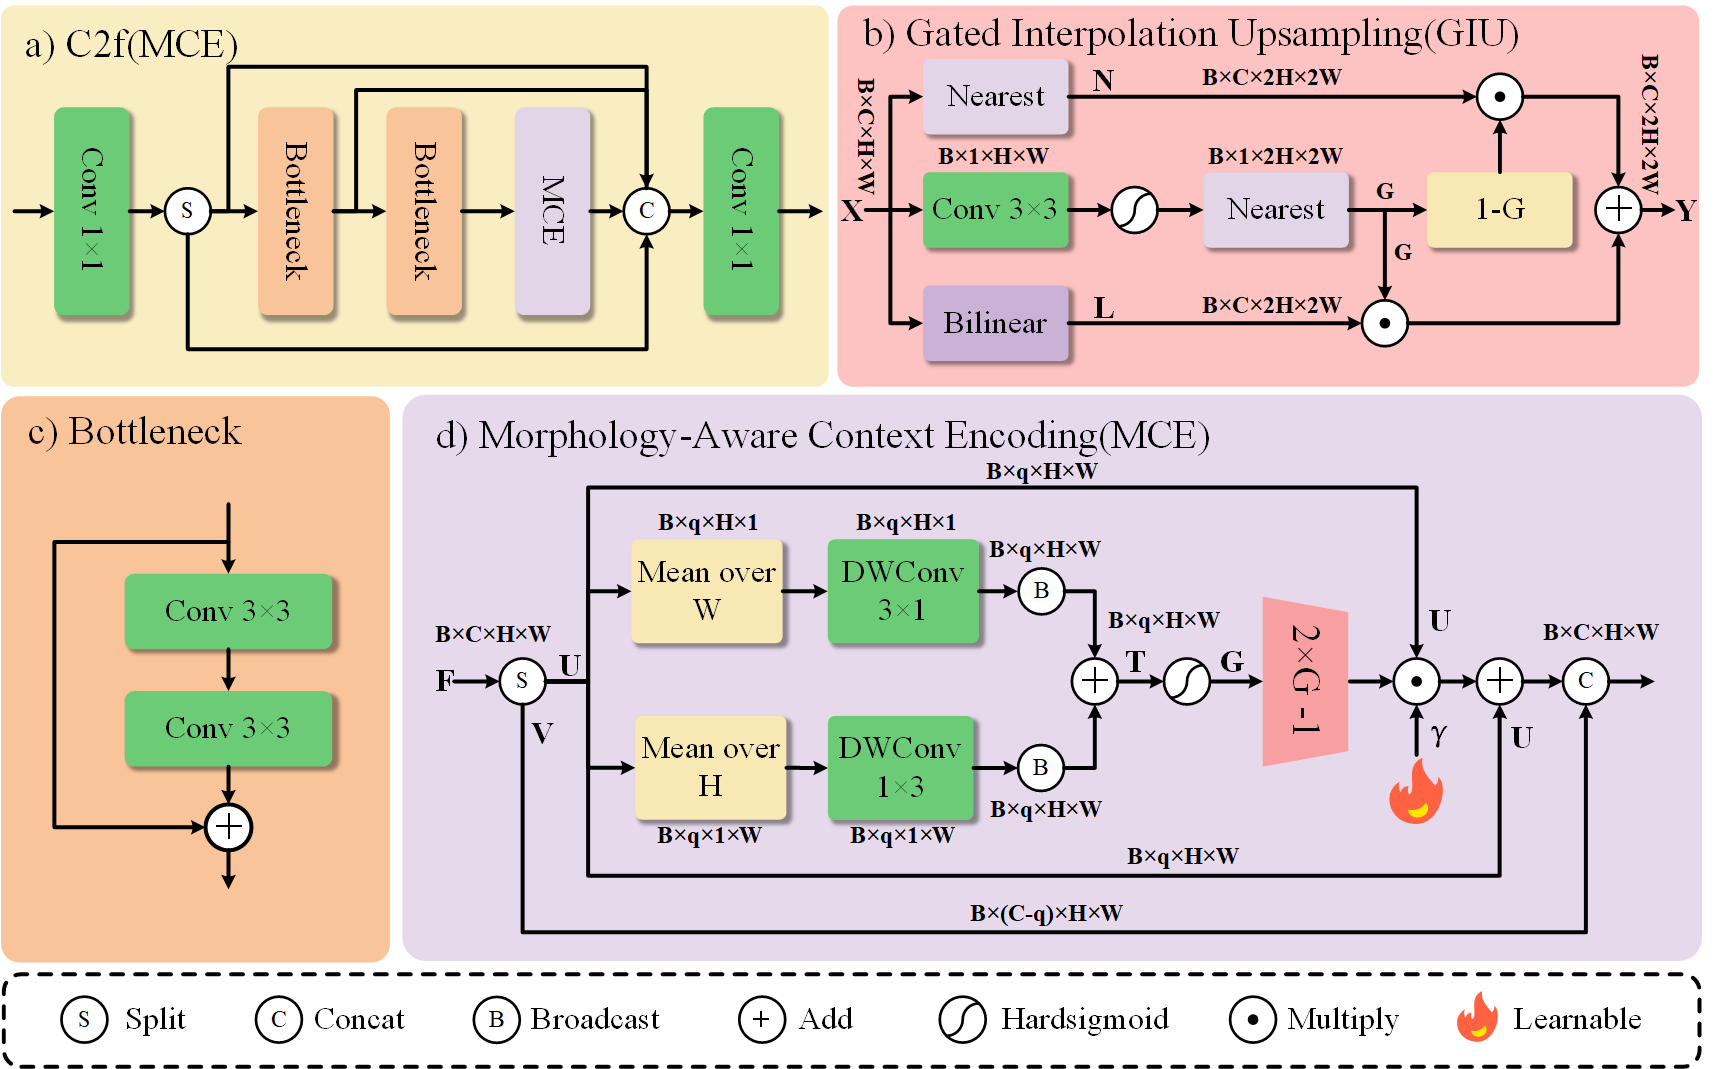
\includegraphics[width=0.9\textwidth]{fig5.png}
\caption{Module structures: (a) MCE-integrated C2f, (b) GIU, (c) bottleneck, and (d) MCE.}
\label{fig:modules}
\end{figure*}

\emph{1) Channel Allocation:}
 As illustrated in Fig.~\ref{fig:modules}(d), its input is $F\in\mathbb{R}^{B\times C\times H\times W}$. The channels are divided into two groups: one quarter of the channels, denoted by $U$, are used for morphology-aware context aggregation and residual modulation; the remaining three quarters, denoted by $V$, pass through unchanged. This design intentionally applies morphology-aware context aggregation to only a small channel subset, keeping the computational overhead compact. The two groups are concatenated after modulation, allowing the subsequent fusion to combine morphology-aware and unmodulated features with minimal performance loss. With $q=C/4$, the two groups have sizes $U\in\mathbb{R}^{B\times q\times H\times W}$ and $V\in\mathbb{R}^{B\times(C-q)\times H\times W}$. The split is performed along the channel dimension, preserving the batch and spatial dimensions.

\emph{2) Morphology-Aware Context Aggregation:}
The one-quarter-channel group $U$ feeds the two pooling paths. Here, $b$, $a$, $h$, and $w$ index the batch sample, channel, row, and column, respectively. Inspired by the pooling design of coordinate attention \cite{hou2021coordinate}, we average independently for each sample and channel:
\begin{align}
R_h(b,a,h,1) &= \frac{1}{W}\sum_{w=1}^{W}U(b,a,h,w), \label{eq:pac-row}\\
R_w(b,a,1,w) &= \frac{1}{H}\sum_{h=1}^{H}U(b,a,h,w), \label{eq:pac-column}
\end{align}
\noindent where averaging over $W$ retains row positions, while averaging over $H$ retains column positions. The descriptors are refined by two depthwise convolutions:
\begin{equation}
\begin{aligned}
D_h&=\operatorname{DW}_{3\times1}(R_h),\\
D_w&=\operatorname{DW}_{1\times3}(R_w),
\end{aligned}
\label{eq:pac-depthwise}
\end{equation}
\noindent where $D_h$ and $D_w$ have sizes $B\times q\times H\times1$ and $B\times q\times1\times W$, respectively. Before addition, $D_h$ is broadcast along $W$ by repeating its column, while $D_w$ is broadcast along $H$ by repeating its row. The expanded features $\widetilde D_h$ and $\widetilde D_w$ both have size $B\times q\times H\times W$ and are added element-wise:
\begin{equation}
T=\widetilde D_h+\widetilde D_w.
\label{eq:pac-context}
\end{equation}

Pooling provides long-range context, while the depthwise convolutions capture neighboring positions in the compressed descriptors.

\emph{3) Residual Context Modulation:}
The combined context $T$ is mapped by Hardsigmoid and centered to construct a scaled residual correction:
\begin{align}
G &= \operatorname{HS}(T), \label{eq:pac-map}\\
U' &= U+\gamma\odot U\odot(2G-1), \label{eq:pac-modulation}
\end{align}
\noindent where $\operatorname{HS}$ is Hardsigmoid, $\odot$ denotes element-wise multiplication with broadcasting, and $\gamma\in\mathbb{R}^{1\times q\times1\times1}$ is a learnable channel-wise parameter. The context response $G\in[0,1]^{B\times q\times H\times W}$ is centered by $2G-1$ to provide signed modulation, with $\gamma$ controlling its channel-wise strength. The original $U$ is retained through the residual connection, and the corrected one-quarter-channel group $U'$ is concatenated with the unchanged three-quarter-channel group $V$. The corrected group has size $U'\in\mathbb{R}^{B\times q\times H\times W}$, and channel concatenation produces a $B\times C\times H\times W$ output before the original C2f fusion. Zero-initializing $\gamma$ makes the module an identity mapping at initialization.

\subsection{Gated Interpolation Upsampling}
Circular-knitting defects vary substantially in morphology and scale, from narrow horizontal and vertical patterns to small and large holes. Their feature representations therefore place different demands on spatial continuity, response concentration, and boundary extent. In the top-down feature pyramid, higher-level context must be reconstructed at a finer resolution before fusion with lateral features. Nearest-neighbor interpolation replicates responses within local regions, whereas bilinear interpolation combines neighboring responses to produce smoother spatial transitions. A fixed interpolation rule applies the same reconstruction behavior to all locations, limiting its adaptability to these diverse defect patterns. We develop GIU to adjust the balance between response replication and neighborhood smoothing according to the input features [Fig.~\ref{fig:modules}(b)]. To achieve this adaptation with a small computational overhead, GIU combines two parameter-free interpolation paths using a single spatial weight map predicted at low resolution and shared across channels. It reconstructs the higher-level context before fusion with shallow lateral features, which retain local texture and localization cues.

\emph{1) Two Fixed Interpolation Paths:}
For $X\in\mathbb{R}^{B\times C\times H\times W}$, nearest-neighbor and bilinear upsampling produce
\begin{align}
N &= \operatorname{Nearest}_{2}(X), \label{eq:giu-paths}\\
L &= \operatorname{Bilinear}_{2}(X), \label{eq:giu-bilinear}
\end{align}
\noindent where $N,L\in\mathbb{R}^{B\times C\times2H\times2W}$. Both operations use fixed interpolation weights and introduce no learnable parameters.

\emph{2) Shared Spatial Gate:}
A $3\times3$ convolution followed by Hardsigmoid predicts a low-resolution spatial weight map, which is then upsampled by nearest-neighbor interpolation:
\begin{align}
g &= \operatorname{HS}(\operatorname{Conv}_{3\times3}(X)), \label{eq:giu-gate-lowres}\\
G &= \operatorname{Nearest}_{2}(g), \label{eq:giu-gate}
\end{align}
\noindent where $\operatorname{Conv}_{3\times3}$ denotes a biased convolution with $C$ input channels, one output channel, and padding of 1, and $g\in[0,1]^{B\times1\times H\times W}$ is the low-resolution weight map. The map $G\in[0,1]^{B\times1\times2H\times2W}$ assigns a content-adaptive interpolation weight to each spatial location and is broadcast across feature channels. Predicting this map at $H\times W$ limits the spatial cost of the learned convolution, while channel sharing requires only one output weight per location.

\emph{3) Gated Reconstruction:}
The output $Y\in\mathbb{R}^{B\times C\times2H\times2W}$ is a convex combination:
\begin{equation}
Y=(1-G)\odot N+G\odot L,
\label{eq:giu-mixture}
\end{equation}
\noindent where small values of $G$ favor response replication, while larger values favor neighborhood smoothing. This spatially varying mixture allows the reconstruction behavior to adapt to local feature content associated with different defect morphologies and scales.
\begin{equation}
G_{\mathrm{init}}=0.05,\qquad Y_{\mathrm{init}}=0.95N+0.05L,
\label{eq:giu-initialization}
\end{equation}
\noindent so the module starts from a predominantly nearest-neighbor reconstruction, consistent with the baseline top-down pathway.

\section{Experiments and Results}
\label{sec:results}
\subsection{Experimental Setup}
\label{sec:experimental-setup}
\subsubsection{Dataset}
The dataset was collected from a real circular-knitting production line and covers three defect categories: horizontal defects (\emph{row}), vertical defects (\emph{col}), and holes (\emph{hole}). It comprises 403 images with 468 annotated defect instances, divided into training, validation, and test sets of 282, 40, and 81 images, respectively, as summarized in Table~\ref{tab:data}. Typical samples and box-morphology distributions are discussed in Section~\ref{sec:defect-morphology}.

\begin{table}[pos=!htbp]
\caption{Dataset split and defect-instance counts.}
\label{tab:data}
\centering
\footnotesize
\begin{tabular}{lrrrrr}
\toprule
Split & Images & Instances & Row & Col & Hole \\
\midrule
Train & 282 & 329 & 174 & 75 & 80 \\
Validation & 40 & 48 & 24 & 13 & 11 \\
Test & 81 & 91 & 60 & 12 & 19 \\
\bottomrule
\end{tabular}
\end{table}

\subsubsection{Implementation Details}
\label{sec:implementation}
Table~\ref{tab:implementation} summarizes the training and deployment settings. \model and its component-ablation variants share the same \texttt{yolov8n.pt} initialization as the YOLOv8n baseline, and all component comparisons use a common training protocol. Other comparison models use available pretrained checkpoints from their respective implementations.

\begin{table}[pos=!htbp]
\caption{Training and edge-deployment settings.}
\label{tab:implementation}
\centering
\footnotesize
\setlength{\tabcolsep}{3pt}
\renewcommand{\arraystretch}{1.08}
\begin{tabular}{@{}P{0.21\columnwidth}P{0.23\columnwidth}P{\dimexpr0.56\columnwidth-12pt\relax}@{}}
\toprule
Category & Parameter & Specification \\
\midrule
\multirow[t]{2}{0.21\columnwidth}{Training setup}
& Hardware & Intel i7-13700KF; NVIDIA RTX 3090 (24 GB) \\
& Software & Ubuntu 24.04, Python 3.10.20, PyTorch 2.4.1+cu124, and Ultralytics 8.4.140 \\
\midrule
\multirow[t]{3}{0.21\columnwidth}{Deployment setup}
& Hardware & Rockchip RK3566 \\
& System & Linux (model evaluation) \\
& Quantization & INT8 \\
\midrule
Data protocol
& Input resolution & Fixed at $640\times640$ \\
\midrule
\multirow[t]{4}{0.21\columnwidth}{Training dynamics}
& Batch & 16  \\
& Maximum epochs & 300 \\
& Patience & 80 epochs \\
& Optimizer & AdamW \\
\bottomrule
\end{tabular}
\renewcommand{\arraystretch}{1.0}
\end{table}

\subsubsection{Evaluation Metrics}
\label{sec:evaluation}
Intersection over union (IoU) measures the overlap between predicted and ground-truth bounding boxes as the ratio of their intersection area to their union area. Precision (P), recall (R), average precision (AP), and mean average precision (mAP) are defined as
\begin{align}
P &= \frac{\mathrm{TP}}{\mathrm{TP}+\mathrm{FP}},
\label{eq:precision}\\
R &= \frac{\mathrm{TP}}{\mathrm{TP}+\mathrm{FN}},
\label{eq:recall}\\
\mathrm{AP} &= \int_0^1 P(R)\,\mathrm{d}R,
\label{eq:ap}\\
\mathrm{mAP} &= \frac{1}{N_c}\sum_{c=1}^{N_c}\mathrm{AP}_c,
\label{eq:metrics}
\end{align}
\noindent where TP, FP, and FN denote true-positive, false-positive, and false-negative counts, respectively; $\mathrm{AP}_c$ is the AP of class $c$, and $N_c=3$. mAP@50 uses an IoU threshold of 0.5, while mAP@50:95 averages mAP over IoU thresholds from 0.50 to 0.95 in steps of 0.05. Reported P and R are averaged across classes, with YOLO-based detectors evaluated at the best mean-F1 operating point. All accuracy metrics are expressed as percentages. In comparison tables, bold and underlined values indicate the best and second-best results, respectively.

Model parameters and FLOPs are measured at $640\times640$ input resolution using each model's respective framework. For FPS comparison, all models are evaluated on an RTX 3090 with FP32 precision, batch size 1, and $640\times640$ inputs. This measurement is separate from the RK3566 deployment result.

\subsection{Comparison With Other Detectors}
Table~\ref{tab:comparison} compares test-set accuracy, model complexity, and inference throughput.

\begin{table*}[width=\textwidth,pos=!tbp]
\caption{Accuracy, complexity, and throughput comparison on the test set.}
\label{tab:comparison}
\centering
\small
\setlength{\tabcolsep}{4pt}
\renewcommand{\arraystretch}{1.06}
\begin{tabular*}{\textwidth}{@{\extracolsep{\fill}}lrrrrrrr}
\toprule
Model & Params (M) & FLOPs (G) & Precision (\%) & Recall (\%) & mAP@50 (\%) & mAP@50:95 (\%) & FPS \\
\midrule
YOLOv9t~\cite{wang2025yolov9} & \textbf{2.12} & 8.5 & 82.4 & 90.8 & 90.1 & 53.3 & 291 \\
YOLOv10n~\cite{wang2024yolov10} & 2.78 & 8.8 & 88.6 & 74.2 & 88.2 & 58.5 & \underline{524} \\
YOLO11n~\cite{ultralytics2023} & 2.62 & \underline{6.7} & 91.1 & 89.5 & 93.3 & 60.8 & 463 \\
YOLO12n~\cite{tian2025yolov12} & 2.60 & 7.6 & 93.0 & 78.5 & 89.0 & 56.8 & 326 \\
YOLO26n~\cite{ultralytics2023} & \underline{2.57} & \textbf{6.2} & 87.3 & 89.4 & 93.8 & 61.1 & 425 \\
RT-DETR-R18~\cite{zhao2024rtdetr} & 20.09 & 60.7 & \textbf{97.7} & \underline{94.5} & 95.2 & \textbf{67.7} & 146 \\
DETR-R50~\cite{carion2020detr} & 41.28 & 77.3 & \textbf{97.7} & \underline{94.5} & 96.4 & 53.6 & 101 \\
Deformable DETR-R50~\cite{zhu2021deformable} & 39.8 & 158.7 & 93.7 & \textbf{97.8} & \underline{96.8} & 64.3 & 49 \\
Faster R-CNN-R50~\cite{ren2015faster} & 41.1 & 181.5 & 95.7 & \textbf{97.8} & 96.1 & 64.7 & 66 \\
YOLOv8n (Baseline)~\cite{ultralytics2023} & 3.01 & 8.1 & 89.4 & 81.1 & 90.5 & 58.4 & \textbf{554} \\
\model & 3.02 & 8.2 & \underline{96.1} & 94.3 & \textbf{97.2} & \underline{65.5} & 486 \\
\bottomrule
\end{tabular*}
\par\smallskip
\renewcommand{\arraystretch}{1.0}
\end{table*}

\begin{figure*}[width=\textwidth,pos=!tbp]
\centering
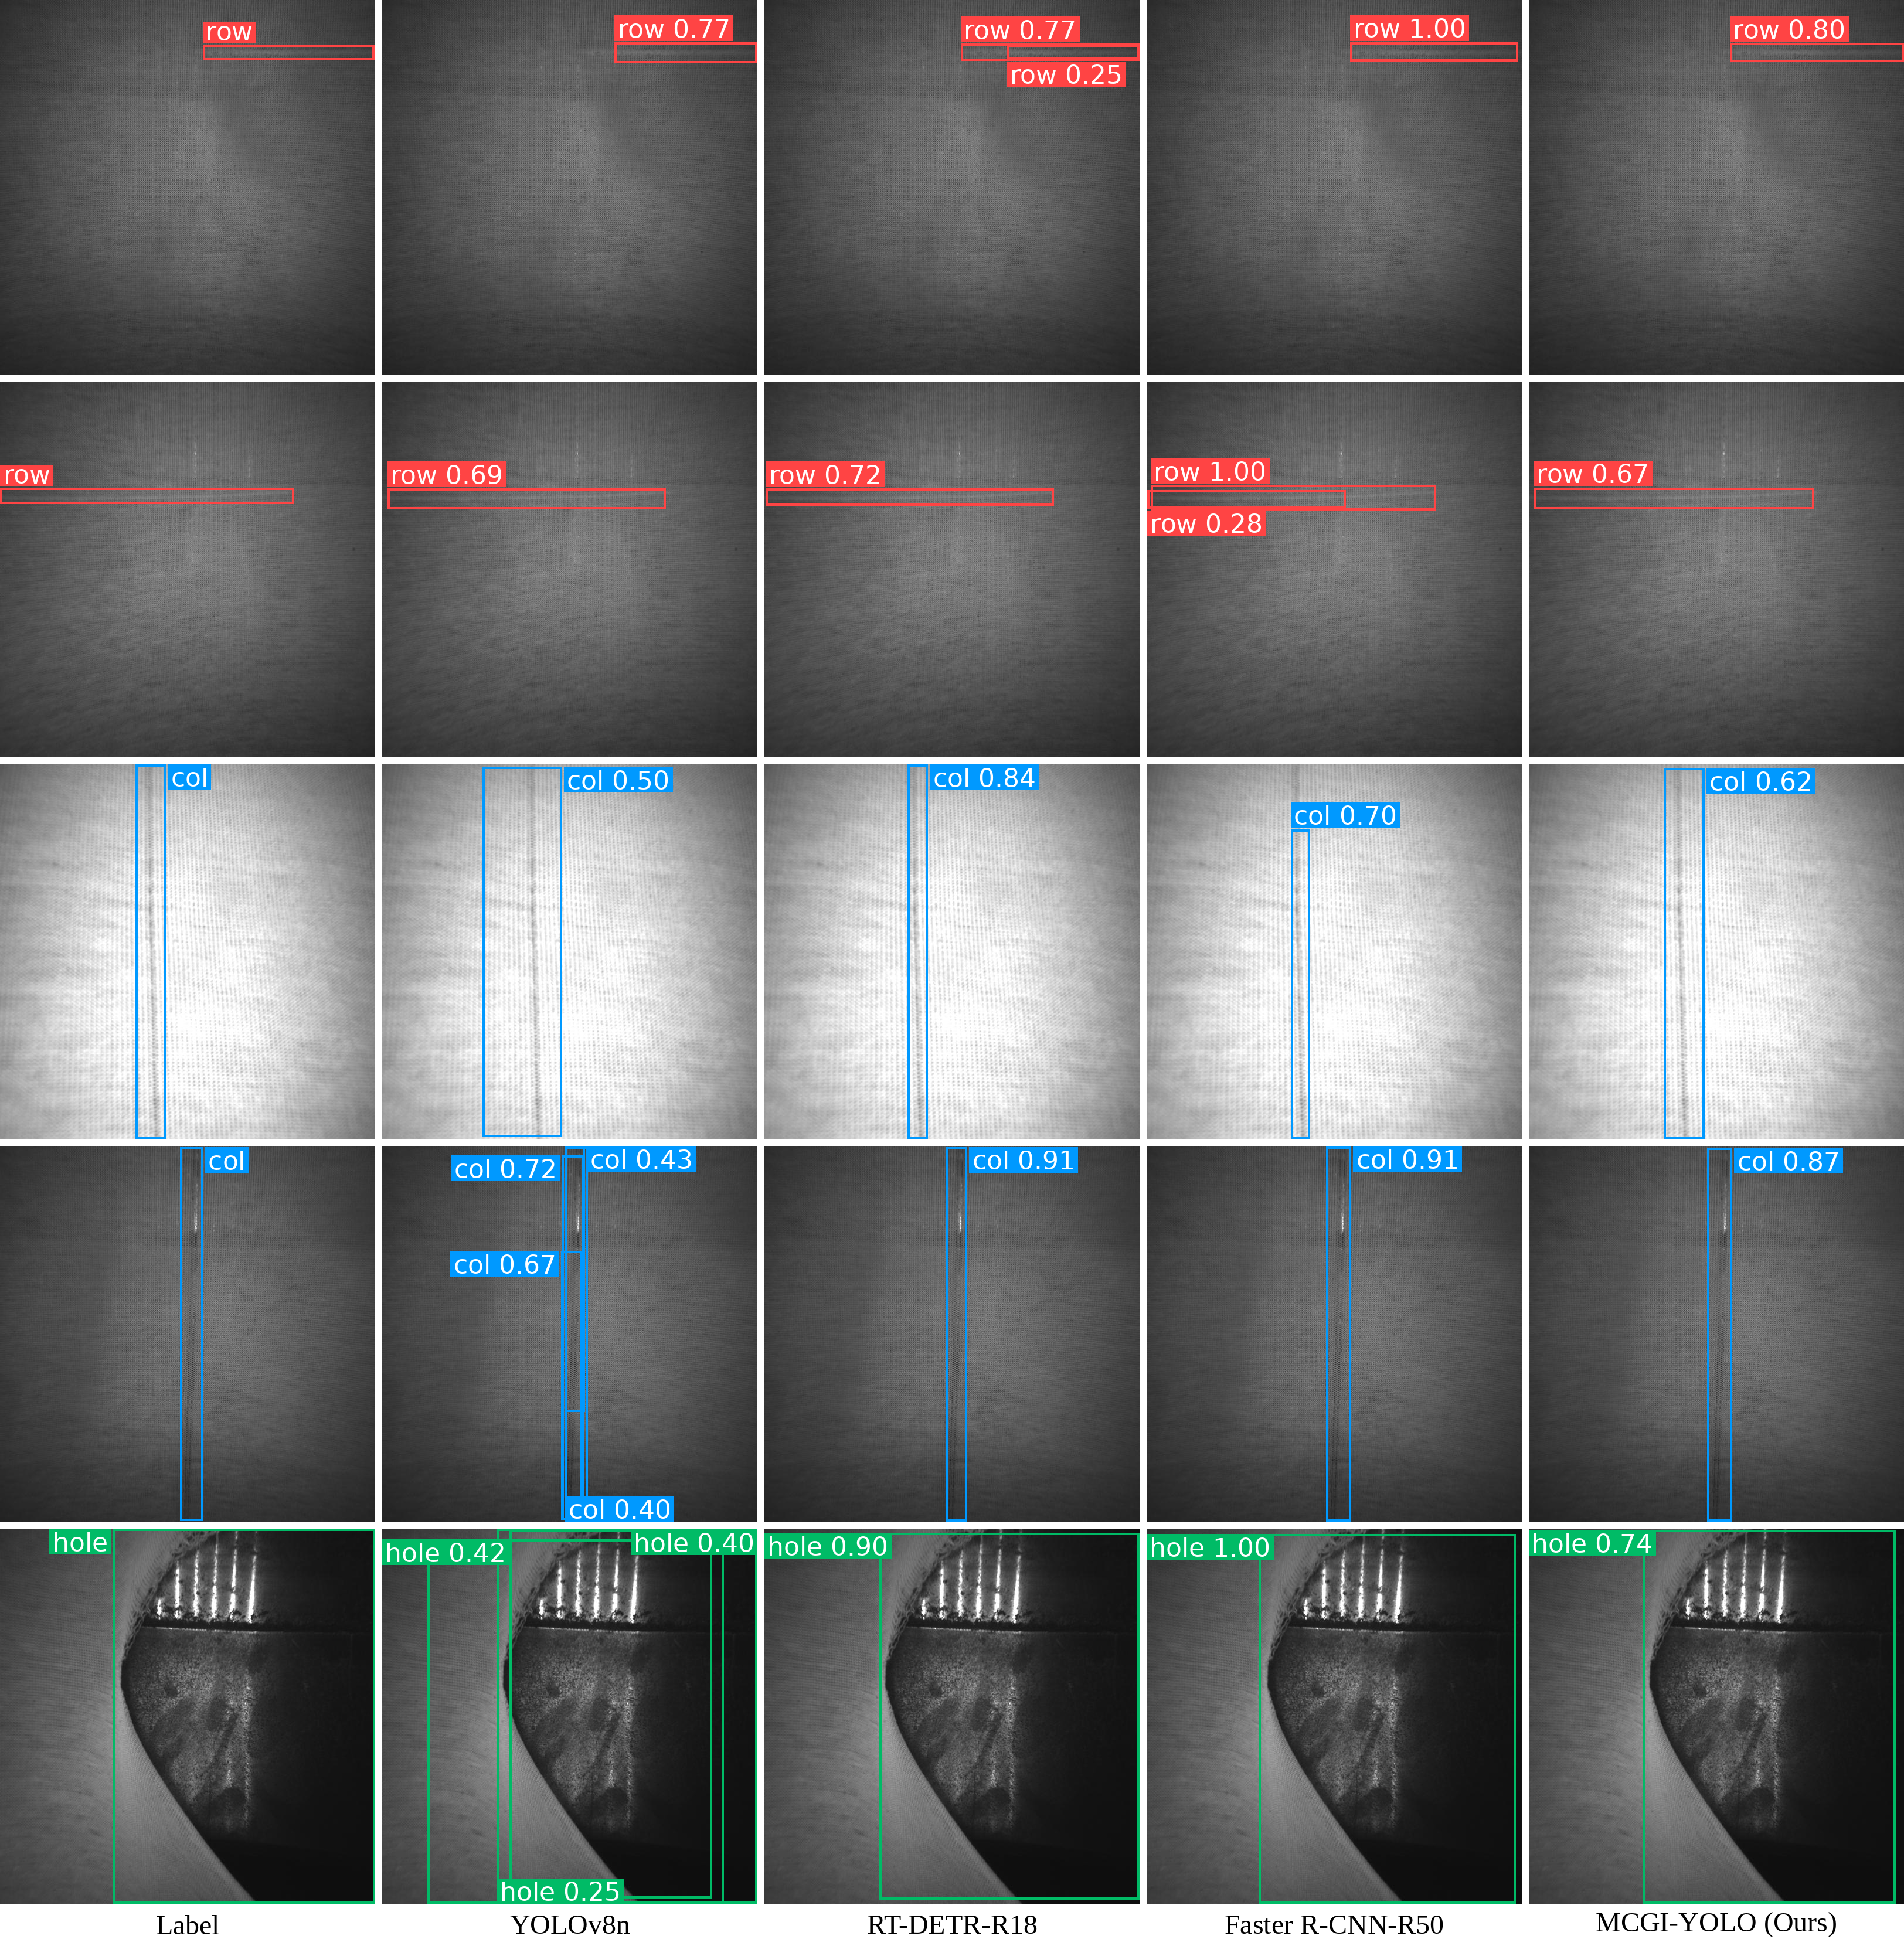
\includegraphics[width=0.86\textwidth]{fig6.png}
\caption{Qualitative comparison of fabric-defect detection results.}
\label{fig:qualitative}
\end{figure*}

\begin{figure*}[width=\textwidth,pos=!tbp]
\centering
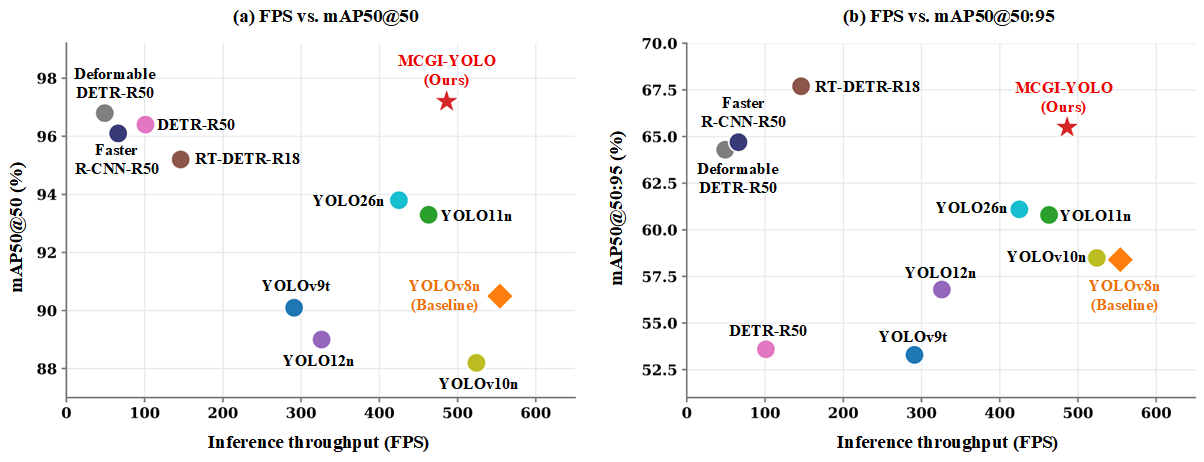
\includegraphics[width=\textwidth]{fps_accuracy.png}
\caption{Accuracy--throughput comparison using (a) mAP@50 and (b) mAP@50:95.}
\label{fig:fps-accuracy}
\end{figure*}

\model achieves the highest mAP@50 of 97.2\% and the second-highest mAP@50:95 of 65.5\%, improving over the YOLOv8n~\cite{ultralytics2023} baseline by 6.7 and 7.1 percentage points, respectively. Its precision and recall are 96.1\% and 94.3\%, exceeding the baseline by 6.7 and 13.2 percentage points, respectively. This gain comes with only a marginal increase in parameters (3.01 M $\rightarrow$ 3.02 M) and FLOPs (8.1 G $\rightarrow$ 8.2 G), while throughput on the RTX 3090 decreases from 554 to 486 FPS. Among lightweight variants, YOLO26n~\cite{ultralytics2023} attains the next-best accuracy (93.8\% mAP@50, 61.1\% mAP@50:95); \model surpasses it by 3.4 and 4.4 points while running faster (486 vs.\ 425 FPS). YOLOv9t~\cite{wang2025yolov9}, YOLOv10n~\cite{wang2024yolov10}, YOLO12n~\cite{tian2025yolov12}, and YOLO26n~\cite{ultralytics2023} have fewer parameters or lower FLOPs but underperform on this test set, confirming that task-specific adaptation outperforms generic lightweight detectors. RT-DETR-R18~\cite{zhao2024rtdetr} leads in mAP@50:95 (67.7\%) but requires 20.09 M parameters and 60.7 G FLOPs at 146 FPS. \model also outperforms DETR-R50~\cite{carion2020detr}, Deformable DETR-R50~\cite{zhu2021deformable}, and Faster R-CNN-R50~\cite{ren2015faster} on both mAP metrics with substantially lower cost. These results indicate that \model provides a favorable balance between detection accuracy and computational complexity, making it suitable for the resource-constrained target platform.

Fig.~\ref{fig:qualitative} shows that \model produces fewer fragmented boxes and tighter localization on elongated defects and holes, consistent with the aggregate results.

Fig.~\ref{fig:fps-accuracy} summarizes the accuracy--throughput tradeoffs for both mAP metrics.

\subsection{Component Ablation}
\label{sec:component-ablation}
\begin{table*}[pos=!tbp]
\caption{Component ablation results.}
\label{tab:ablation}
\label{tab:ablation-classwise}
\centering
\fontsize{8}{9.5}\selectfont
\setlength{\tabcolsep}{3pt}
\begin{tabular*}{\textwidth}{@{\extracolsep{\fill}}lrrrrrrrrrr@{}}
\toprule
\multirow{2}{*}{Variant} & \multirow{2}{*}{\shortstack{Params\\(M)}} & \multirow{2}{*}{\shortstack{FLOPs\\(G)}} & \multicolumn{2}{c}{Overall (\%)} & \multicolumn{2}{c}{Row (\%)} & \multicolumn{2}{c}{Col (\%)} & \multicolumn{2}{c}{Hole (\%)} \\
\cmidrule(lr){4-5}\cmidrule(lr){6-7}\cmidrule(lr){8-9}\cmidrule(lr){10-11}
& & & mAP@50 & mAP@50:95 & AP@50 & AP@50:95 & AP@50 & AP@50:95 & AP@50 & AP@50:95 \\
\midrule
YOLOv8n & 3.01 & 8.10 & 90.5 & 58.4 & 98.2 & 62.7 & 82.8 & 52.7 & \underline{90.4} & 59.7 \\
YOLOv8n + MCE & 3.01 & 8.2 & 93.9 & \underline{63.6} & \textbf{99.4} & \textbf{65.3} & 93.2 & \underline{64.7} & 89.1 & 60.9 \\
YOLOv8n + GIU & 3.01 & 8.2 & \underline{94.4} & 63.0 & \underline{99.0} & \underline{64.5} & \underline{96.6} & 61.9 & 87.8 & \underline{62.6} \\
\model & 3.02 & 8.2 & \textbf{97.2} & \textbf{65.5} & 98.7 & 64.4 & \textbf{99.5} & \textbf{66.9} & \textbf{93.5} & \textbf{65.2} \\
\bottomrule
\end{tabular*}
\end{table*}

Table~\ref{tab:ablation} compares four configurations on the same 81 test images containing 91 defects under a common evaluation protocol. MCE alone retains nearest-neighbor upsampling, while GIU alone retains the original backbone C2f blocks. MCE increases Row and Col AP@50:95 by 2.6 and 12.0 percentage points, respectively, consistent with using extended directional context to associate spatially separated elongated-defect responses. GIU improves AP@50:95 for Row, Col, and Hole by 1.8, 9.2, and 2.9 points, respectively, consistent with its content-adaptive reconstruction for shape and scale variation. However, Hole AP@50 decreases from 90.4\% to 89.1\% with MCE and 87.8\% with GIU alone.

Combining the modules achieves the highest Col and Hole AP@50 (99.5\% and 93.5\%) and AP@50:95 (66.9\% and 65.2\%). The latter exceed the best single-module results by 2.2 and 2.6 points, respectively. This pattern suggests that MCE supplies more coherent contextual features and GIU adapts their reconstruction before fusion with local features, benefiting both elongated Col defects and localized holes. The interaction is class-dependent: Row AP@50:95 is 64.4\%, below the MCE-only result of 65.3\%. Fig.~\ref{fig:heatmaps} provides corresponding feature visualizations.



\begin{table*}[pos=!tbp]
\caption{Comparisons with reference modules.}
\label{tab:reference-modules}
\centering
\fontsize{8}{9.5}\selectfont
\setlength{\tabcolsep}{3pt}
\begin{tabular*}{\textwidth}{@{\extracolsep{\fill}}lrrrrrrrrrr@{}}
\toprule
\multirow{2}{*}{Module} & \multirow{2}{*}{\shortstack{Params\\(M)}} & \multirow{2}{*}{\shortstack{FLOPs\\(G)}} & \multicolumn{2}{c}{Overall (\%)} & \multicolumn{2}{c}{Row (\%)} & \multicolumn{2}{c}{Col (\%)} & \multicolumn{2}{c}{Hole (\%)} \\
\cmidrule(lr){4-5}\cmidrule(lr){6-7}\cmidrule(lr){8-9}\cmidrule(lr){10-11}
& & & mAP@50 & mAP@50:95 & AP@50 & AP@50:95 & AP@50 & AP@50:95 & AP@50 & AP@50:95 \\
\midrule
\multicolumn{11}{l}{Context encoding: nearest-neighbor upsampling fixed} \\
CA~\cite{hou2021coordinate} & 3.0088 & \textbf{8.1} & \textbf{93.4} & \textbf{56.3} & 97.5 & 56.9 & \textbf{87.3} & 50.7 & \textbf{95.2} & \textbf{61.4} \\
MCE & \textbf{3.0064} & \textbf{8.1} & 88.5 & \textbf{56.3} & \textbf{98.4} & \textbf{60.6} & 81.2 & \textbf{53.8} & 85.8 & 54.5 \\
\midrule
\multicolumn{11}{l}{Upsampling: original C2f backbone fixed} \\
Bilinear & \textbf{3.0062} & \textbf{8.1} & 92.3 & 59.1 & 97.3 & \underline{61.6} & 89.6 & 58.6 & \textbf{89.9} & 57.2 \\
CARAFE~\cite{wang2019carafe} & 3.1463 & 8.4 & \underline{94.3} & \underline{61.7} & \textbf{99.4} & 61.1 & \textbf{97.2} & \textbf{65.4} & 86.4 & \underline{58.6} \\
GIU & \underline{3.0097} & \textbf{8.1} & \textbf{94.4} & \textbf{63.0} & \underline{99.0} & \textbf{64.5} & \underline{96.6} & \underline{61.9} & \underline{87.8} & \textbf{62.6} \\
\bottomrule
\end{tabular*}
\end{table*}

Table~\ref{tab:reference-modules} adds reference comparisons using seed 1 and the same test set and evaluation protocol. CA and MCE occupy the same P3/P4 C2f insertion sites with nearest-neighbor upsampling fixed; Bilinear, CARAFE, and GIU replace both top-down upsampling operations with the original backbone retained. Complexity values are taken from the fused-model evaluation summaries. Both CA and MCE report 56.3\% mAP@50:95. MCE achieves higher Row and Col AP@50:95 (60.6\% and 53.8\%, versus 56.9\% and 50.7\%), consistent with its directional-continuity prior. CA has higher overall mAP@50 (93.4\% versus 88.5\%) and Hole AP@50:95 (61.4\% versus 54.5\%).

GIU achieves 63.0\% mAP@50:95, exceeding Bilinear and CARAFE by 3.9 and 1.3 percentage points, respectively. Its Row and Hole AP@50:95 exceed CARAFE by 3.4 and 4.0 points, while CARAFE performs better on Col (65.4\% versus 61.9\%). GIU uses 3.0097 M parameters and 8.1 G reported FLOPs, compared with CARAFE's 3.1463 M and 8.4 G. These results support content-adaptive interpolation for heterogeneous defect morphologies with a small learned-parameter overhead.

\begin{figure}[pos=!htbp]
\centering
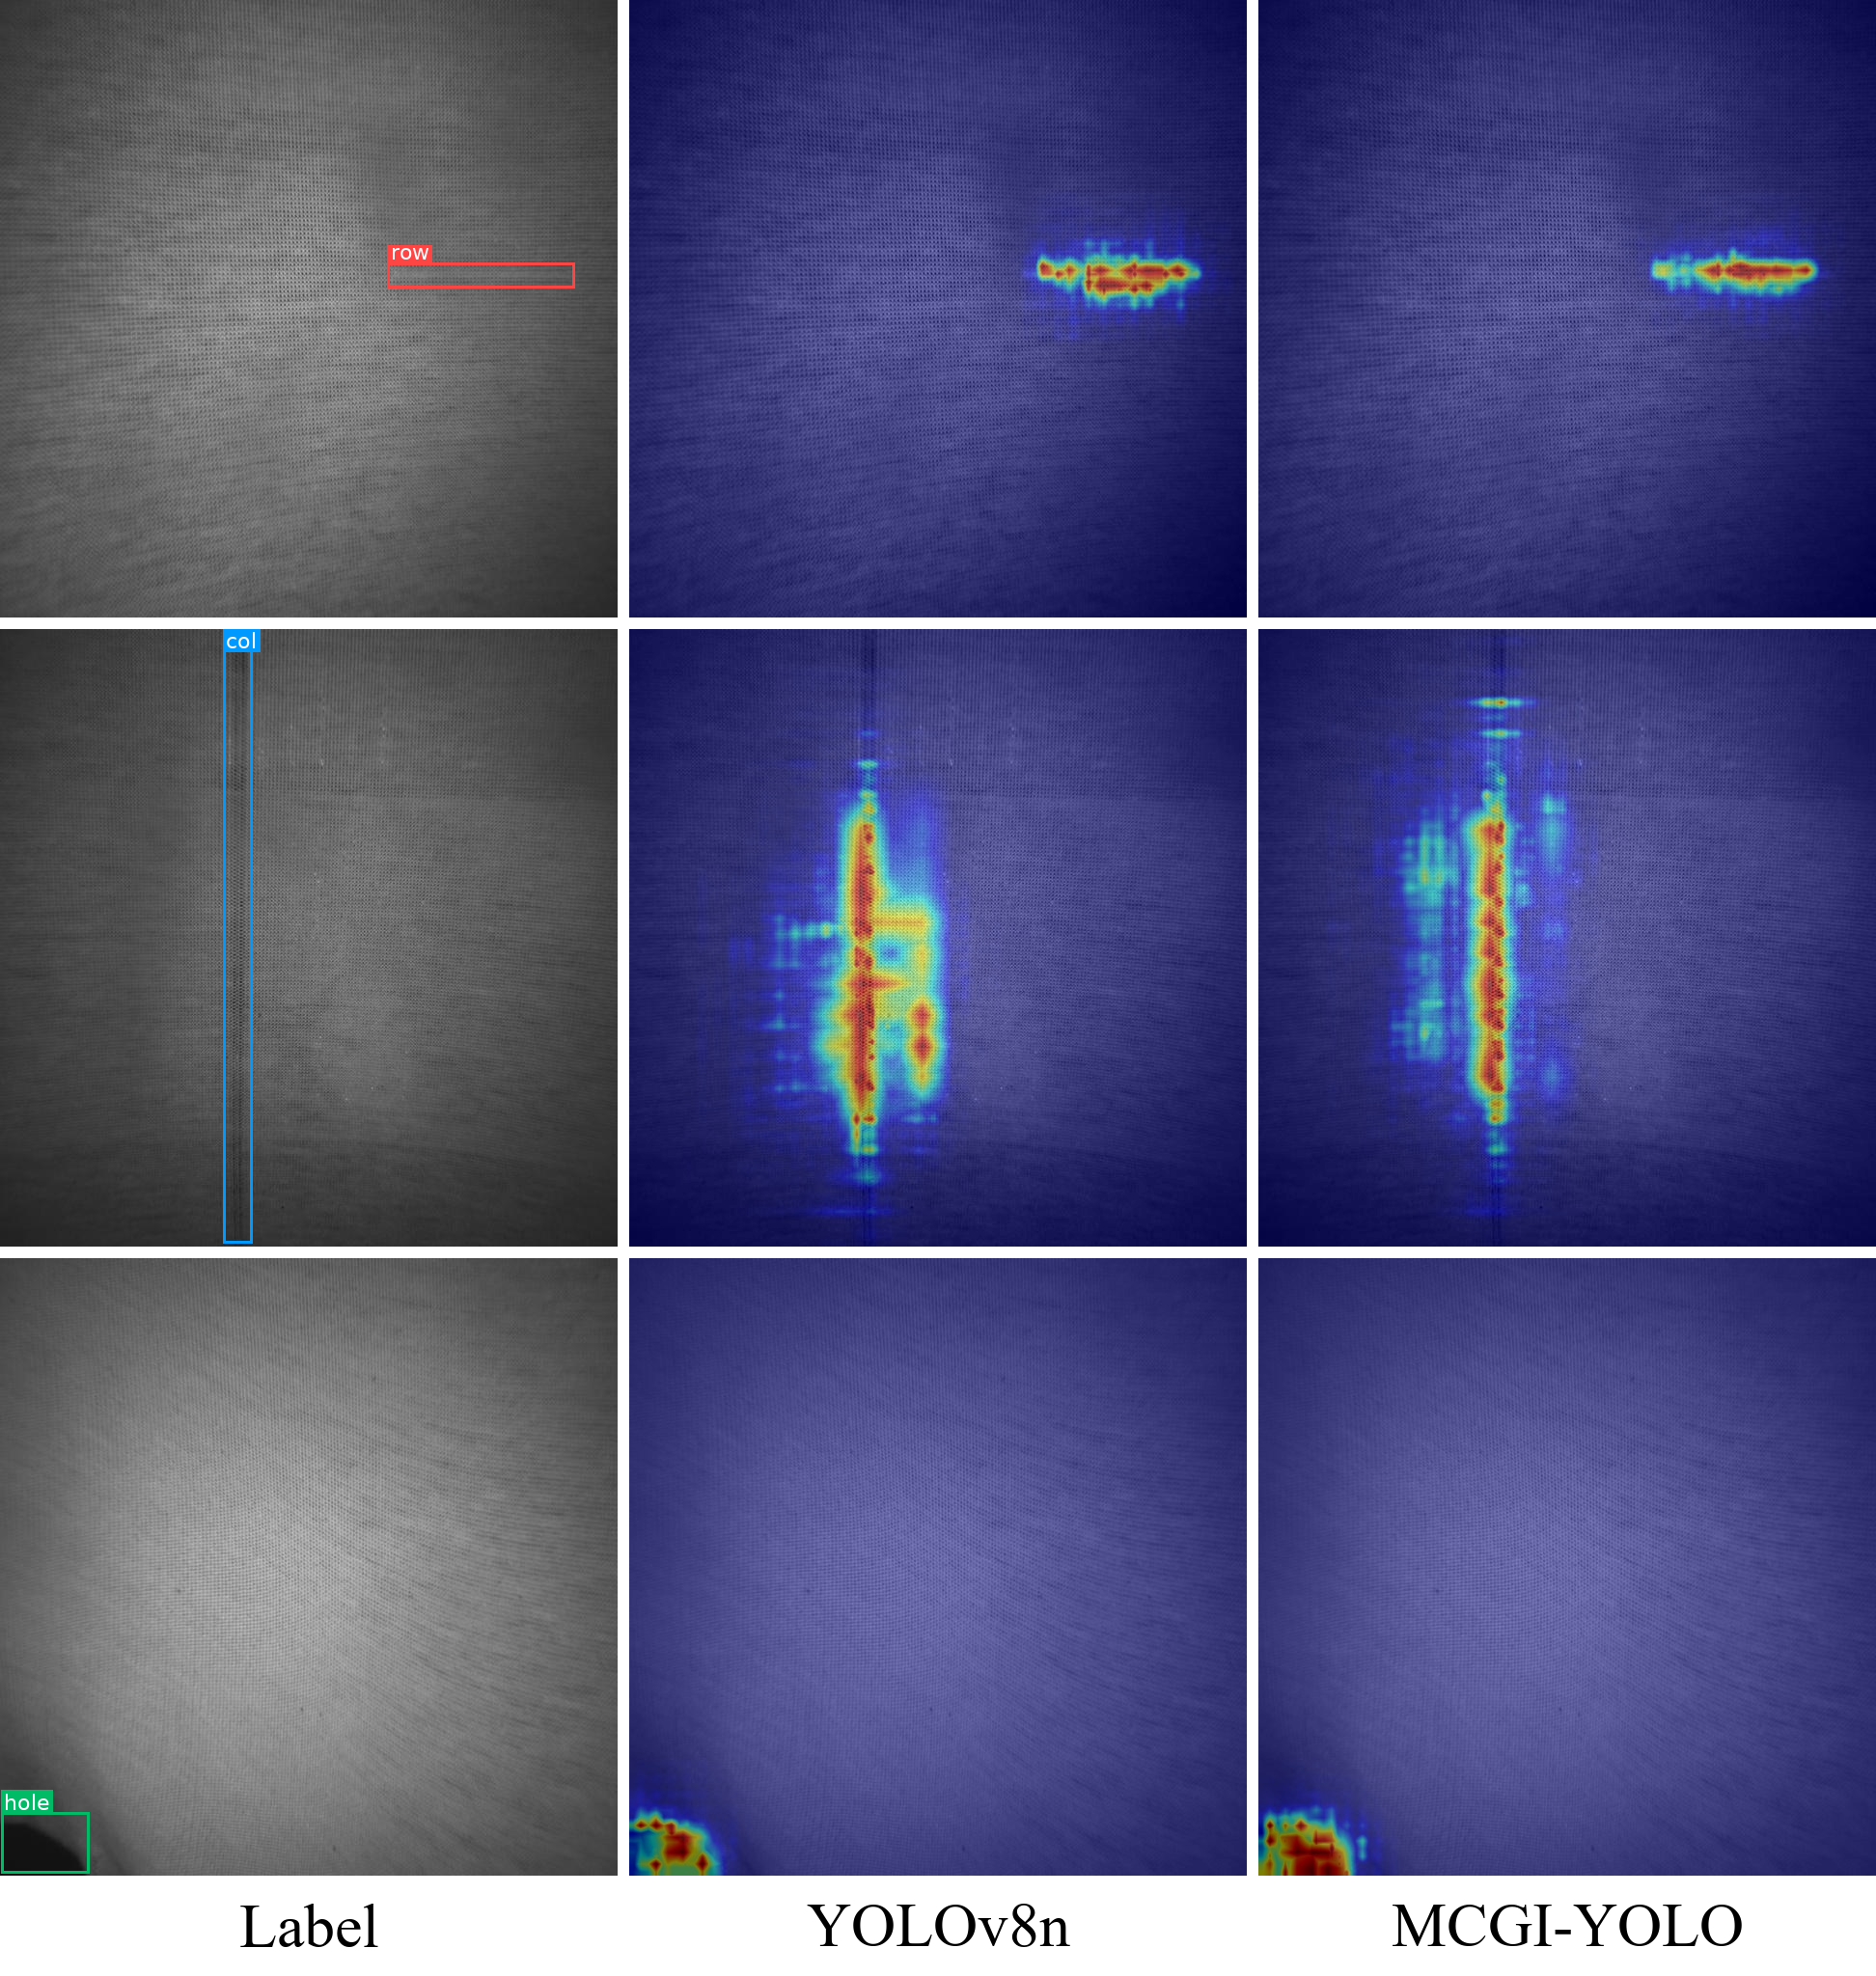
\includegraphics[width=\columnwidth]{fig7.png}
\caption{Feature visualizations of YOLOv8n and \model.}
\label{fig:heatmaps}
\end{figure}

\section{System Deployment and Industrial Application}
\label{sec:system-operation}
The inspection workflow is implemented through the dedicated edge device, client interface, cloud platform, and configurable stopping rules. This section evaluates on-device inference and closed-loop response, and describes configurable stopping decisions, local intervention, remote supervision, operator feedback, and the resulting change in factory inspection practice.

\subsection{Model Deployment and On-Device Performance}
\label{sec:deployment}
To deploy \model on the RK3566 edge device, the trained model is exported to ONNX with a fixed input size of $640\times640$ and then converted into an INT8 RKNN model using RKNN-Toolkit2 \cite{rockchiptoolkit2}. The converted \model and YOLOv8n baseline are evaluated under Linux on the same 81 test images with 91 annotated defects. Both models use a prediction confidence cutoff of 0.001, an NMS IoU threshold of 0.7, and a maximum of 16 detections per image.

Table~\ref{tab:rknn-deployment} reports the deployed models' overall detection accuracy and inference throughput. \model achieves 96.685\% mAP@50 and 64.020\% mAP@50:95, exceeding the deployed YOLOv8n baseline by 6.492 and 6.730 percentage points, respectively. Its overall precision and recall reach 97.599\% and 93.001\%. Relative to the PyTorch results in Table~\ref{tab:comparison}, the deployed \model shows reductions of 0.515 and 1.480 percentage points in the two mAP metrics. On the RK3566, YOLOv8n and \model achieve model-inference throughputs of 30 and 23 FPS, respectively. The latter is 2.3 times the 10 FPS design target derived in Section~\ref{sec:coverage}, meeting the model-inference rate required for the specified machine speed and camera field of view.

\begin{table}[pos=!htbp]
\caption{Accuracy and throughput of INT8 models deployed on the RK3566.}
\label{tab:rknn-deployment}
\centering
\footnotesize
\setlength{\tabcolsep}{2pt}
\renewcommand{\arraystretch}{1.08}
\begin{tabular*}{\columnwidth}{@{\extracolsep{\fill}}lrrrrr@{}}
\toprule
Model & P & R & mAP@50 & mAP@50:95 & FPS \\
\midrule
YOLOv8n & 88.323 & 81.316 & 90.193 & 57.290 & \textbf{30} \\
\textbf{\model} & \textbf{97.599} & \textbf{93.001} & \textbf{96.685} & \textbf{64.020} & 23 \\
\bottomrule
\end{tabular*}
\renewcommand{\arraystretch}{1.0}
\end{table}

\subsubsection{Closed-Loop Response Time}
\label{sec:closed-loop-response}
For a frame that triggers stopping, timing starts at preprocessing entry and ends when the machine is stationary, excluding image acquisition and SerDes transmission. The total response time is
\begin{equation}
\begin{aligned}
T_{\mathrm{total}}={}&T_{\mathrm{pre}}+T_{\mathrm{infer}}+T_{\mathrm{post}}\\
&+T_{\mathrm{cmd}}+T_{\mathrm{stop}},
\end{aligned}
\label{eq:closed-loop-response}
\end{equation}
\noindent where $T_{\mathrm{pre}}=25$ ms, $T_{\mathrm{infer}}=43.5$ ms, $T_{\mathrm{post}}=7$ ms, and $T_{\mathrm{cmd}}=36$ ms denote the measured preprocessing, inference, postprocessing with stopping decision, and command-execution times, respectively. Successive stage boundaries are model input readiness, model output availability, stopping-decision completion, and stop-signal issuance.

The software stages total 111.5 ms before the stop signal is issued. Including the typical machine-braking interval $T_{\mathrm{stop}}=1.5$--$1.8$ s gives an estimated total response of 1.61--1.91 s. Thus, the local stop command is issued in approximately 0.11 s, while the reported 23 FPS characterizes model inference only.

\subsection{User-Configurable Post-NMS Stopping Decision}
\label{sec:stop-rules}
Textile factories differ in their tolerance for fabric defects and the quality requirements of their products. We therefore introduce a user-configurable postprocessing stage after non-maximum suppression (NMS), translating detection results into machine-stop decisions. Three editable sensitivity presets, low, medium, and high, accommodate different factory acceptance criteria.

Each sensitivity preset combines a confidence threshold, three geometric thresholds, and a defect-count threshold per frame, as listed in Table~\ref{tab:stop-rules}.

\begin{table}[pos=!htbp]
\caption{User-configurable machine-stop parameters.}
\label{tab:stop-rules}
\centering
\footnotesize
\setlength{\tabcolsep}{3pt}
\renewcommand{\arraystretch}{1.08}
\begin{tabular*}{\columnwidth}{@{\extracolsep{\fill}}lrrrrr@{}}
\toprule
Level & $\tau_s$ & \shortstack{$A_s$\\(pixels$^2$)} & \shortstack{$W_s$\\(pixels)} & \shortstack{$H_s$\\(pixels)} & $N_s$ \\
\midrule
Low & 0.50 & 6400 & 800 & 400 & 3 \\
Medium & 0.40 & 2500 & 400 & 200 & 2 \\
High & 0.30 & 1000 & 200 & 100 & 1 \\
\bottomrule
\end{tabular*}
\renewcommand{\arraystretch}{1.0}
\end{table}

Class-aware NMS suppresses redundant overlapping predictions within each category. The retained bounding boxes are mapped back to the original $1280\times1024$ camera image before their dimensions are evaluated. For sensitivity level $s$, let $\tau_s$ denote the confidence threshold, $W_s$ and $H_s$ the horizontal- and vertical-defect length thresholds in pixels, $A_s$ the hole-area threshold in square pixels, and $N_s$ the defect-count threshold. For detection $i$ with class $c_i$, bounding-box width $w_i$, and height $h_i$, the geometric qualification indicator is
\begin{equation}
r_i^{(s)}=
\begin{cases}
1, & c_i=\mathrm{row},\quad w_i>W_s\\
1, & c_i=\mathrm{col},\quad h_i>H_s\\
1, & c_i=\mathrm{hole},\quad w_i h_i>A_s\\
0, & \text{otherwise}
\end{cases},
\label{eq:stop-rule}
\end{equation}
\noindent where $r_i^{(s)}=1$ indicates that the detection exceeds its class-specific size threshold; otherwise, $r_i^{(s)}=0$. Width measures the horizontal extent of a row defect, height measures the vertical extent of a column defect, and bounding-box area measures the extent of a hole. Let $\mathcal{P}$ denote the detections retained by NMS and $p_i$ the confidence of detection $i$. The set $\mathcal{D}_s=\{i\in\mathcal{P}\mid p_i\geq\tau_s\}$ contains the confidence-qualified detections in the current frame. The stopping decision is
\begin{equation}
S_s=
\begin{cases}
1, & \displaystyle\sum_{i\in\mathcal{D}_s}r_i^{(s)}\geq1\\
1, & |\mathcal{D}_s|\geq N_s\\
0, & \text{otherwise}
\end{cases},
\label{eq:frame-stop-rule}
\end{equation}
\noindent where $S_s=1$ triggers a stop command, and $S_s=0$ continues inspection. A stop command is issued when either a confidence-qualified detection exceeds its class-specific size threshold or the total number of confidence-qualified detections reaches $N_s$. The count criterion includes defects below the geometric thresholds, allowing multiple small defects to trigger stopping. Counts are evaluated independently for each frame.

Higher sensitivity lowers the confidence, size, and count thresholds, allowing stopping for smaller defects or fewer detections within a frame. Lower sensitivity raises these thresholds to accommodate less stringent acceptance criteria. The editable presets convert detection outputs into factory-specific production decisions without retraining the detector.

\subsection{Client Detection Interface and Operator Feedback}
\label{sec:client-interface}
An Android client application is developed in Kotlin and deployed on the RK3566 edge device, providing detection-state visualization, sensitivity configuration, defect review, and operator feedback.

Fig.~\ref{fig:client-detection} shows the detection home page (left), defect-review interface (center), and mobile notification interface (right). The home page displays the detection state, device information, and current sensitivity setting. Upon defect detection, the client automatically switches to the defect-detail page, displaying the captured image, the localized defect, and its category for operator review. The confirmation buttons on the right side of the defect-detail page allow the operator to indicate whether the detected defect warrants machine stopping under the factory's quality requirements. These assessments link detection images and results to operator feedback, providing samples for review, annotation, and subsequent model refinement.

\begin{figure*}[width=\textwidth,pos=!tbp]
\centering
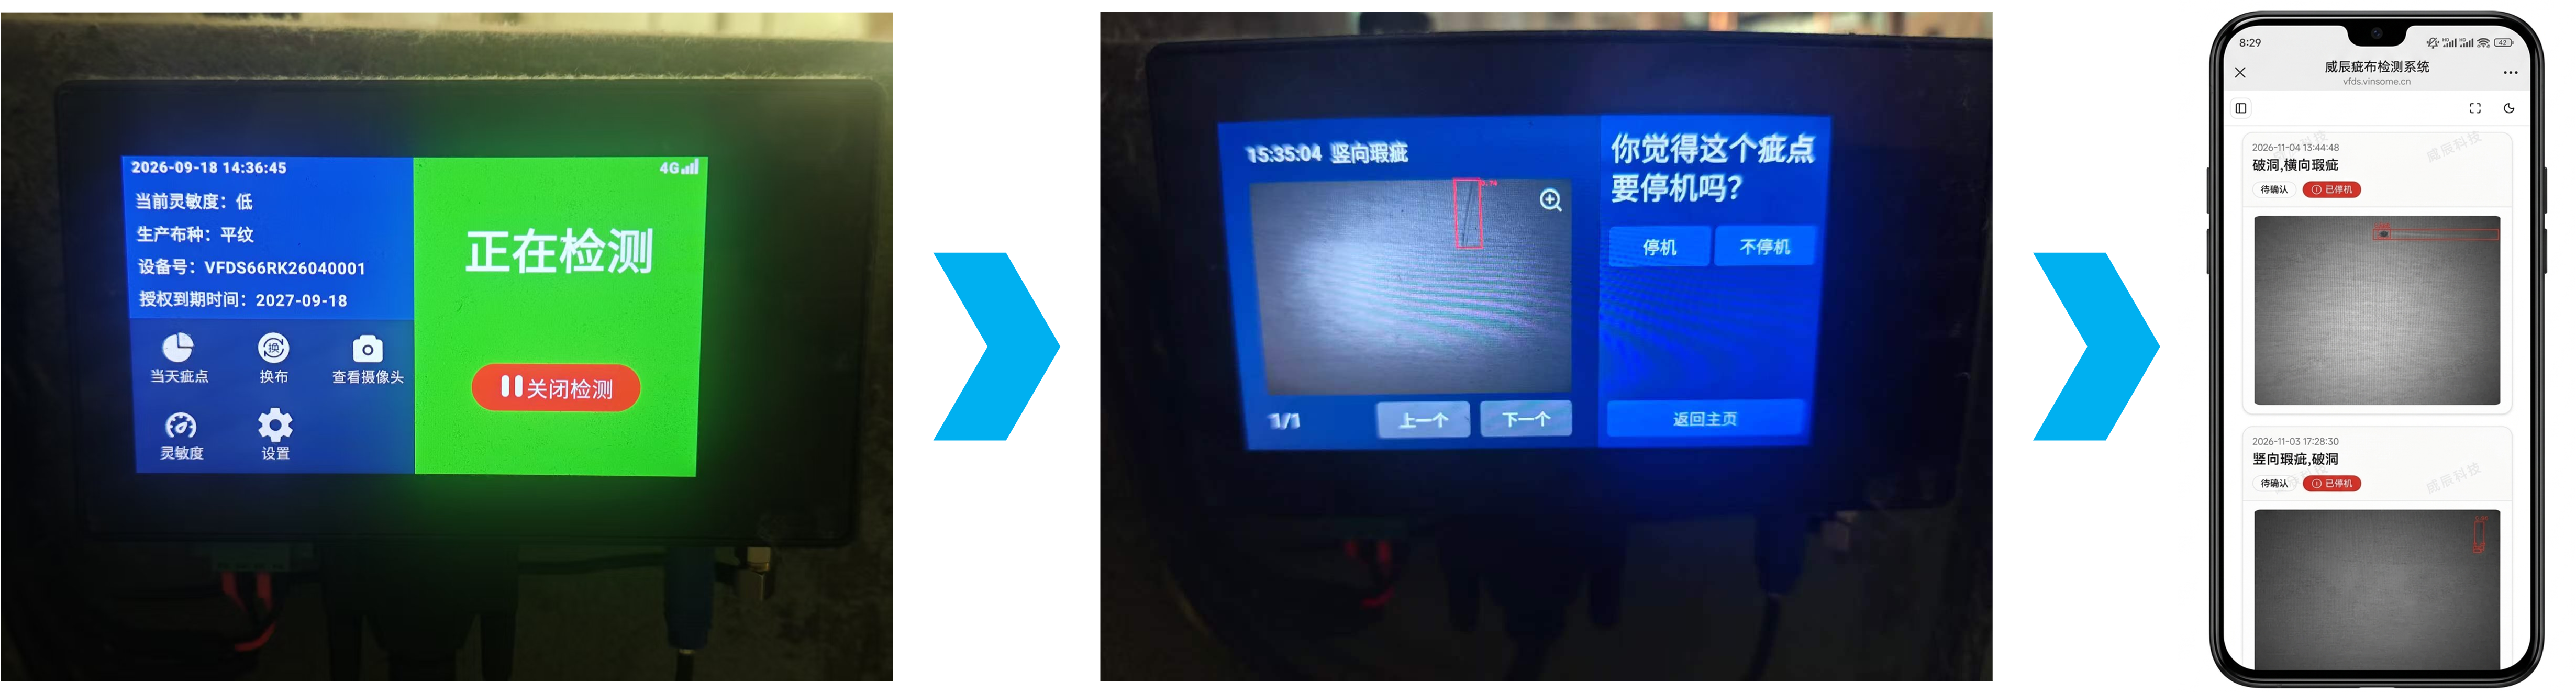
\includegraphics[width=0.98\textwidth]{detect.png}
\caption{Client detection, defect review, and mobile notification interfaces.}
\label{fig:client-detection}
\end{figure*}

\subsection{Cloud Monitoring and Remote Management}
\label{sec:network-client}
The edge device reports defect events and runtime states to the cloud and receives remote configuration updates. Local detection and machine-stop commands are executed on the edge device, while the cloud provides centralized monitoring and management.

The system landing page, defect trends, and defect records are shown in Fig.~\ref{fig:iot-platform}(a)--(c), respectively. The runtime-state interface in Fig.~\ref{fig:iot-platform}(f) displays the application version, camera status, CPU temperature, fabric type, and detection state. The configuration interface in Fig.~\ref{fig:iot-platform}(d) supports remote adjustment of sensitivity and the associated confidence, geometric, and defect-count thresholds.

The model-management interface in Fig.~\ref{fig:iot-platform}(e) accepts RKNN models and associated class-label files for on-demand over-the-air (OTA) model updates. Updated models can be distributed remotely to edge devices for subsequent local inference. Operator feedback, model refinement, and OTA redeployment thus form an iterative improvement workflow that incorporates production experience into model updates.

\begin{figure*}[width=\textwidth,pos=!tbp]
\centering
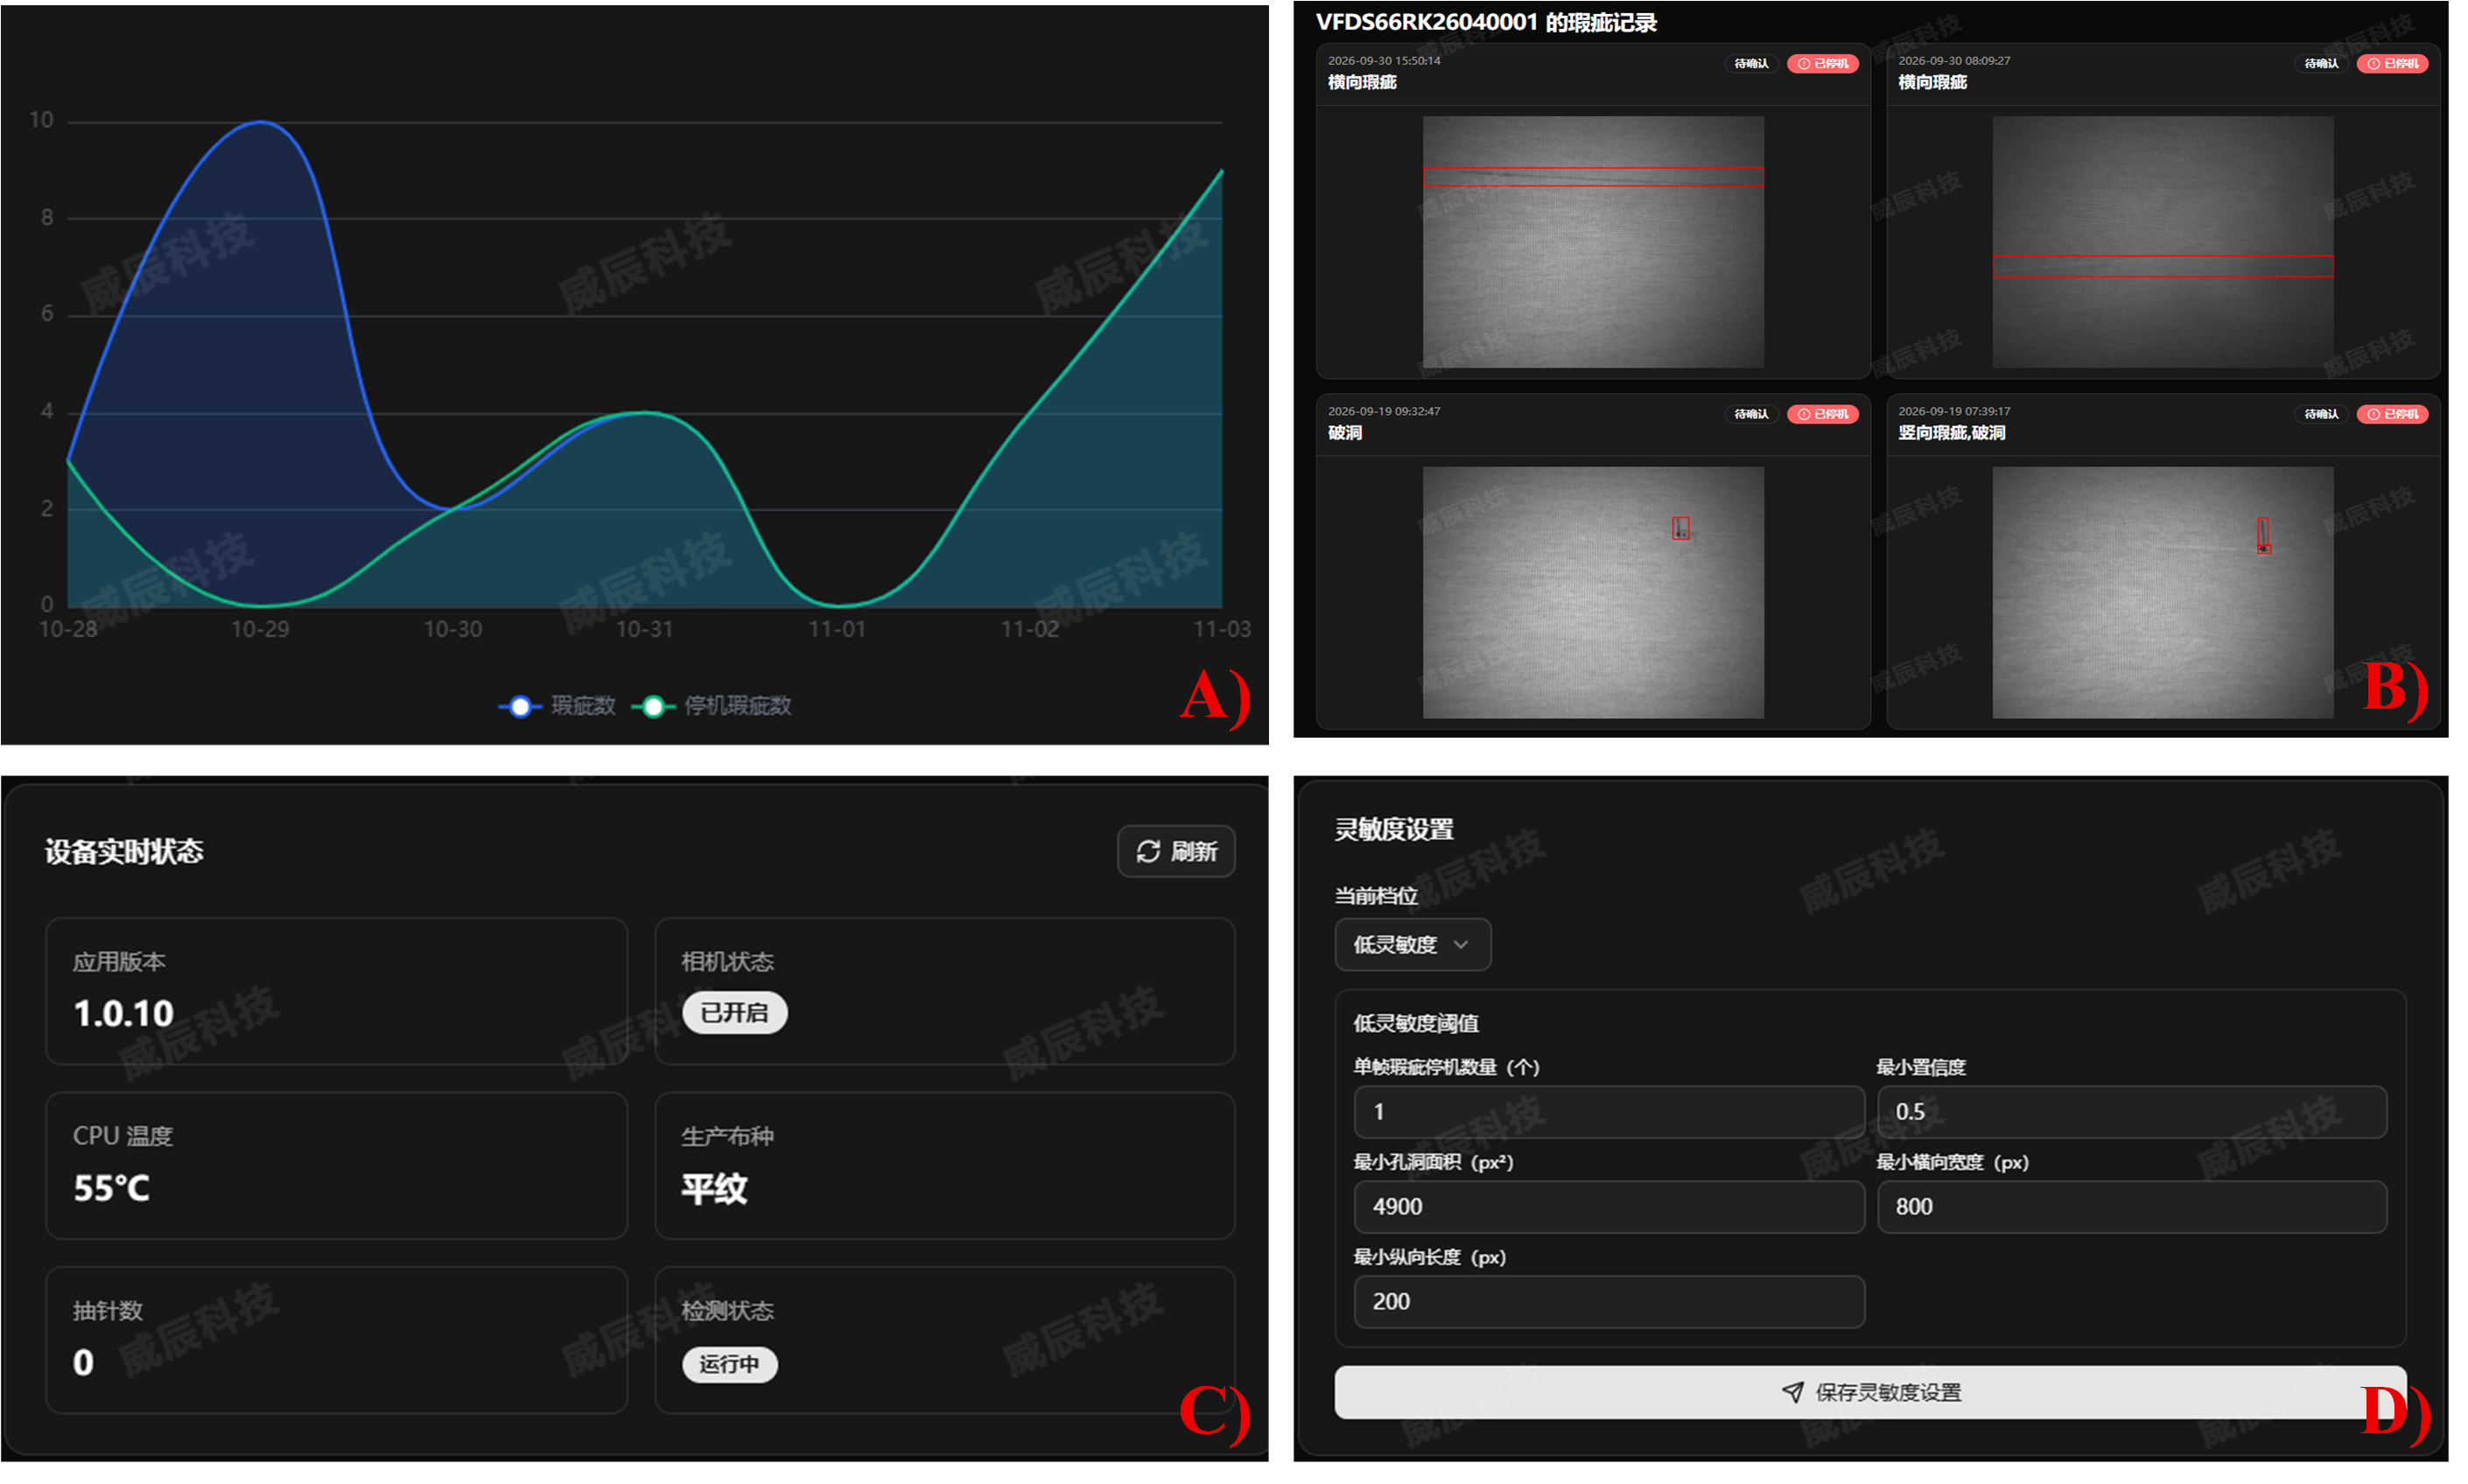
\includegraphics[width=0.98\textwidth]{iot_platform.png}
\caption{IoT platform for monitoring and remote management.}
\label{fig:iot-platform}
\end{figure*}

\subsection{Rule Configuration and Stop Execution}
The client applies the post-NMS stopping decision defined in Section~\ref{sec:stop-rules} to each processed frame. Operators can select a sensitivity preset and edit the confidence, geometric, and count thresholds locally. The same parameters can be updated remotely through the interface in Fig.~\ref{fig:iot-platform}(D). When the stopping condition is met, the edge device issues a local machine-stop command and uploads the defect event for cloud recording and operator notification.

\subsection{Illustrative Analysis of Defect Propagation Before Intervention}
\label{sec:delayed-intervention}
Fig.~\ref{fig:waste-fabric} shows actual waste fabric with repeated horizontal defects caused by a yarn abnormality. When the abnormality persists at an active feeder, a new defective course can be generated on each machine revolution, following the course-formation mechanism of circular weft knitting \cite{cottonworksKnitMachinery}. Without timely detection and intervention, these horizontal defects recur as the fabric is knitted and taken down, extending the affected region along the production direction and causing the affected fabric to be discarded.

\begin{figure}[pos=!htbp]
\centering
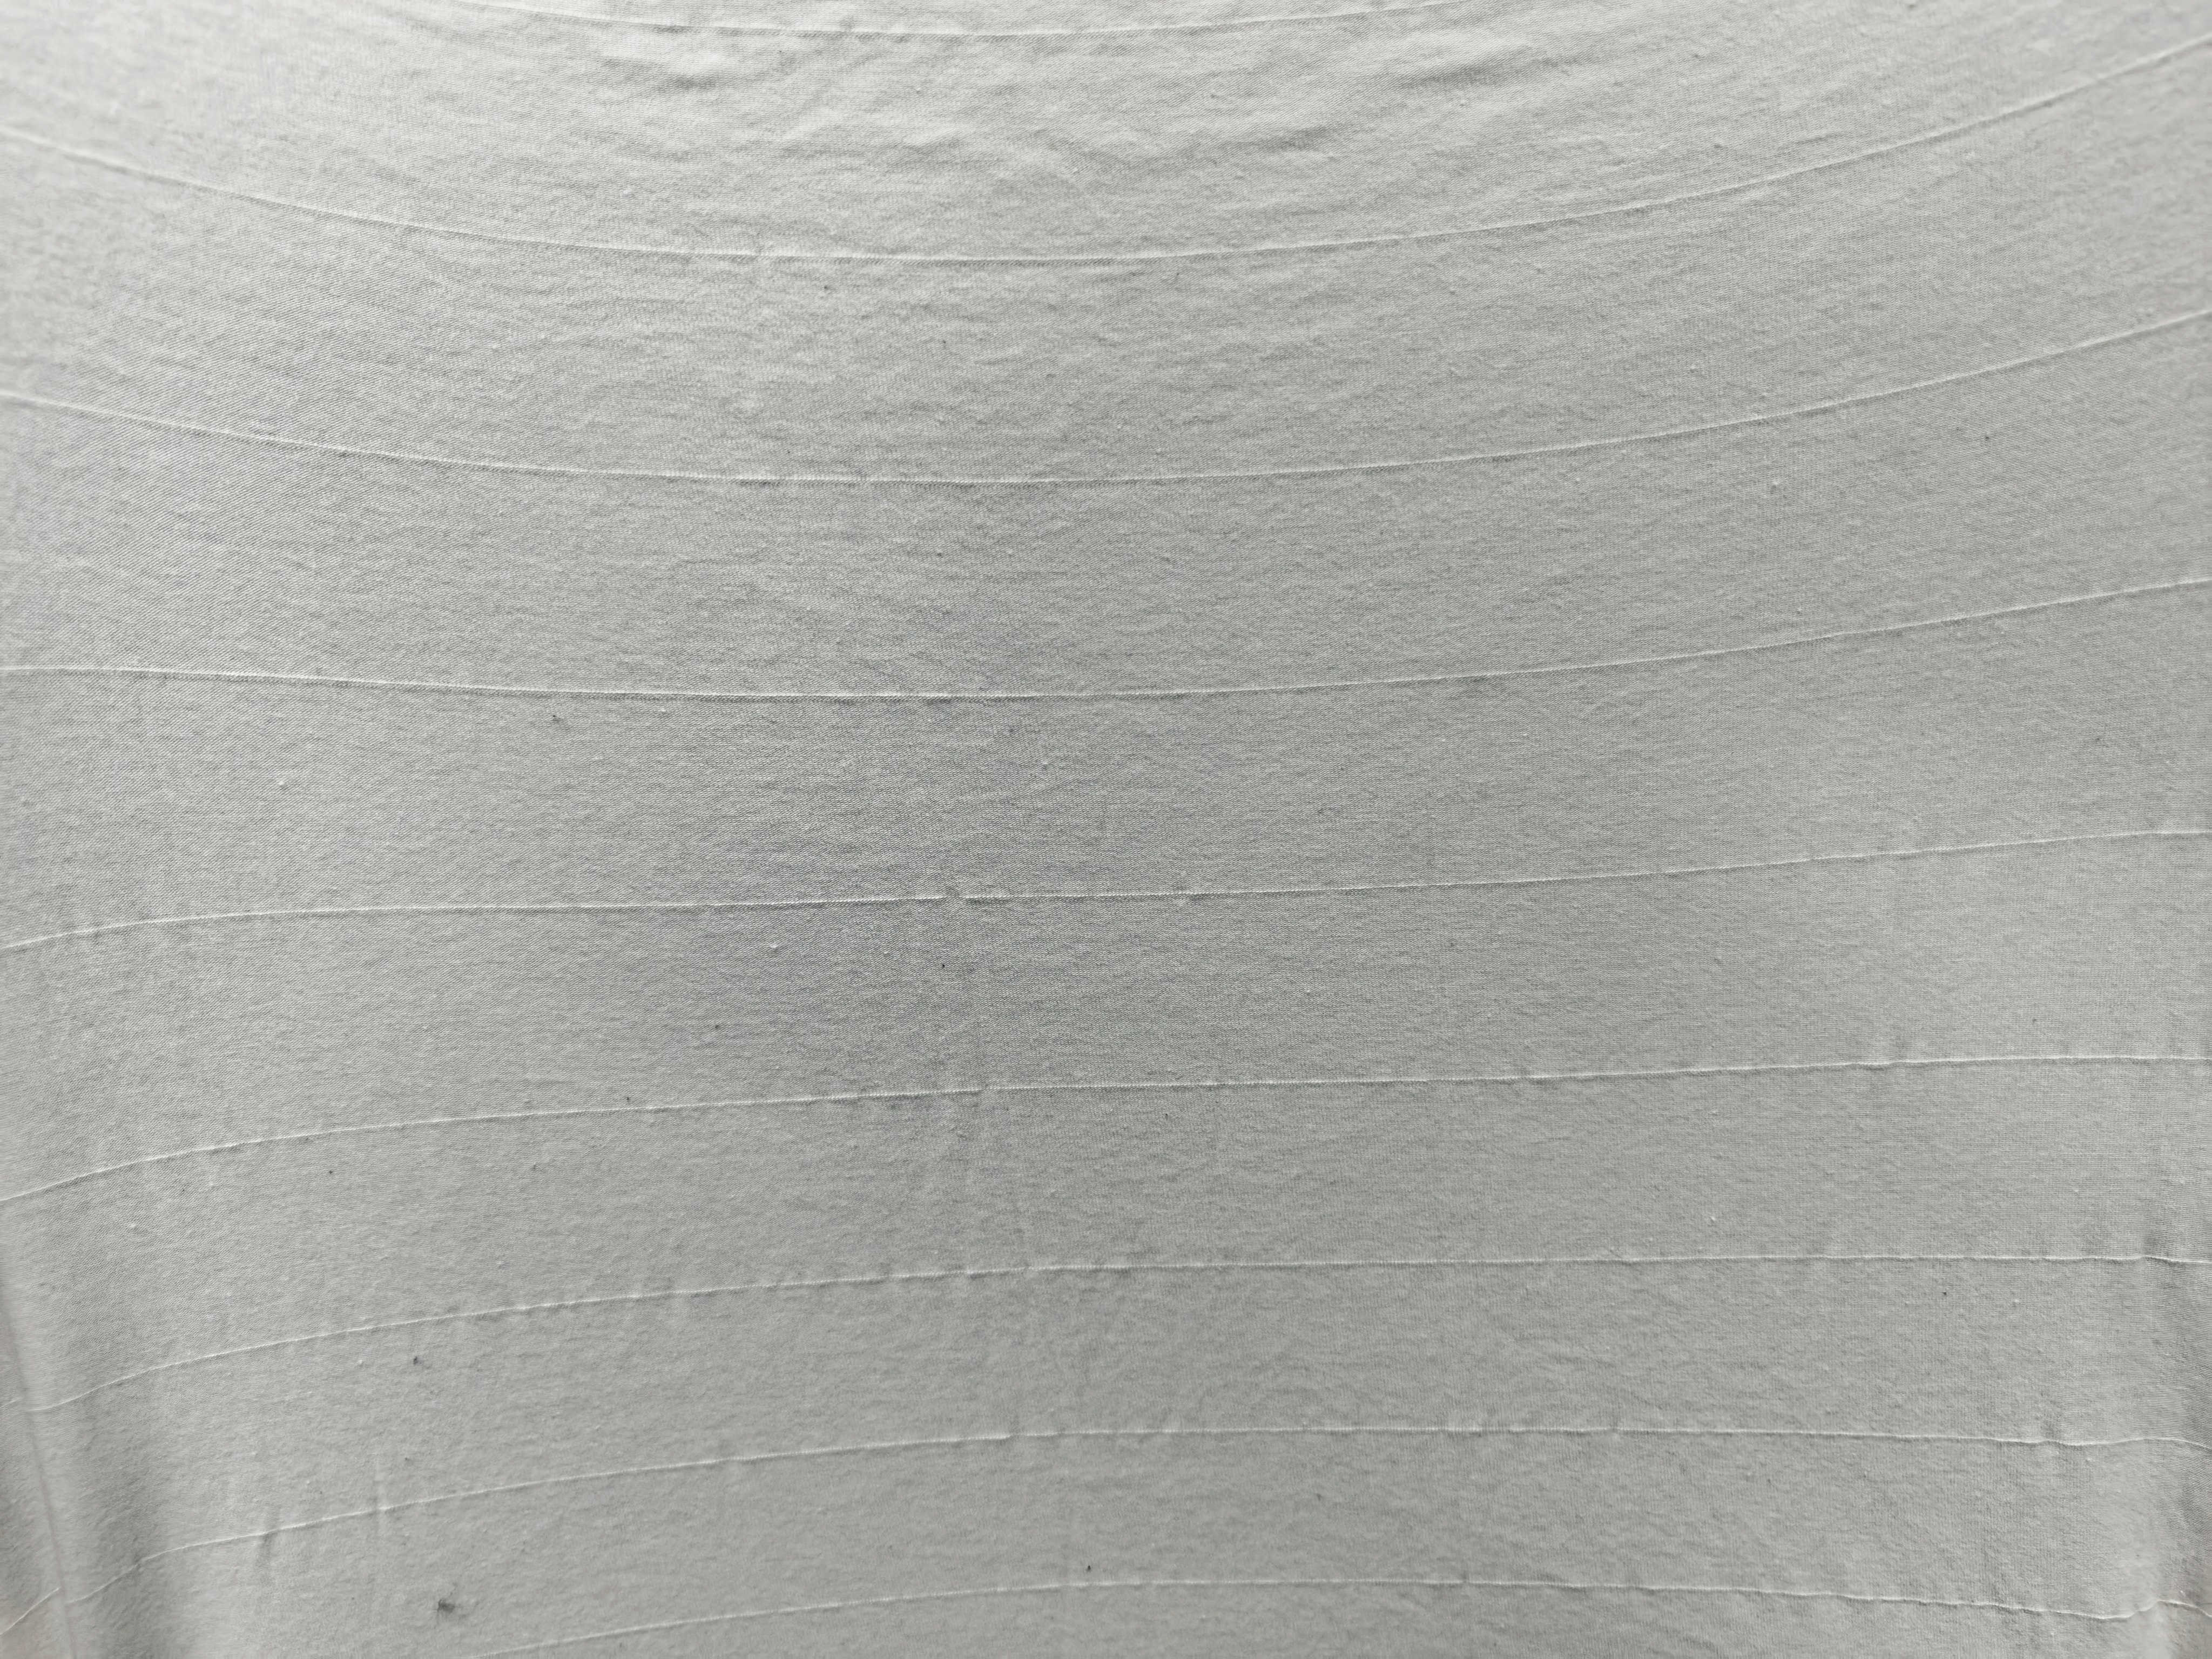
\includegraphics[width=0.9\columnwidth]{fabric_with_defect.jpg}
\caption{Waste fabric with recurring horizontal defects.}
\label{fig:waste-fabric}
\end{figure}

Consider a three-minute delay ($\tau=180$ s) between defect onset and operator discovery. The machine completes $N=\tau/T=90$ revolutions during this interval. Assuming that each revolution produces a horizontal defect extending approximately around the fabric circumference, the sum of these transverse defect lengths is
\begin{equation}
L_{\mathrm{sum}}=N\pi D
=90\times\pi\times1.016
\approx287.3\ \mathrm{m}.
\label{eq:cumulative-defect-length}
\end{equation}

\Needspace{5\baselineskip}
The corresponding affected fabric length in the production direction is determined by the take-down increment, taken as $p=0.03$ m per revolution:
\begin{equation}
L_{\mathrm{affected}}=Np
=\frac{180}{2}\times0.03
\approx2.7\ \mathrm{m}.
\label{eq:affected-fabric-length}
\end{equation}

These estimates describe approximately 2.7 m of affected fabric in the production direction, containing 90 repeated horizontal defects with a summed transverse length of 287.3 m. The latter measures accumulated defect extent across revolutions, rather than the length of discarded fabric.

\subsection{Factory Application and Waste Reduction}
\label{sec:factory-benefits}
The system is applied at our collaborating factory, Dongguan Minghai Textile Co., Ltd., Dongguan, Guangdong, China, which operates 48 circular knitting machines and reports an approximate monthly fabric output of 350 t. Table~\ref{tab:factory-benefits} compares factory-provided monthly estimates of fabric waste and losses before and after deployment. The estimated monthly fabric waste decreases by 92.7\%, with the waste rate falling from 0.580\% before deployment to 0.042\% after deployment. The resulting net fabric-loss reduction is approximately USD 5637.68 per month, or USD 67,652.21 on an annualized basis.

\begin{table}[pos=!htbp]
\caption{Estimated monthly fabric waste and losses before and after deployment.}
\label{tab:factory-benefits}
\centering
\footnotesize
\setlength{\tabcolsep}{3pt}
\renewcommand{\arraystretch}{1.08}
\begin{tabular*}{\columnwidth}{@{\extracolsep{\fill}}lrr@{}}
\toprule
Indicator & Before & After \\
\midrule
Number of machines & 48 & 48 \\
Monthly fabric waste (kg) & $\approx2030$ & $\approx148$ \\
Net material loss (USD/kg) & 3.00 & 3.00 \\
Estimated monthly fabric loss (USD) & 6081.03 & 443.35 \\
Monthly loss per machine (USD) & 126.69 & 9.24 \\
\bottomrule
\end{tabular*}
\renewcommand{\arraystretch}{1.0}
\par\smallskip
\begin{minipage}{\columnwidth}
\footnotesize
Normal fabric and waste recovery values are USD 3.74/kg and USD 0.75/kg, respectively.
\end{minipage}
\end{table}

For an illustrative procurement scenario, a publicly documented project specifies 2000 circular knitting machines and 160 opening-and-inspection machines \cite{xinjing2024eia}. Applying this ratio to 48 knitting machines and rounding up yields a reference configuration of four inspection machines. At a reference unit price of USD 2522.28, their combined procurement budget would be approximately USD 10,089.12. Whether this expenditure can be avoided depends on actual purchase plans and the remaining need for finished-fabric inspection, including checks for downstream defects, grading, and customer acceptance. No cancellation of equipment purchases has been verified at the collaborating factory; this reference budget is therefore excluded from the reported monthly and annualized material-loss reductions. The on-machine workflow directs operator attention to reported defects and production faults.

\section{Conclusion}
\label{sec:conclusion}
This paper presents an inspection workflow that embeds fabric-defect detection and intervention in circular-knitting production. The dedicated system coordinates rotation-activated detection, continuous image acquisition, SerDes transmission, edge inference, configurable machine stopping, and operator notification. Its lightweight detector, \model, combines MCE for elongated-defect continuity with GIU for adaptive feature reconstruction. On the production-line test set, it achieves 97.2\% mAP@50 and 65.5\% mAP@50:95, improving over YOLOv8n by 6.7 and 7.1 percentage points. INT8 deployment achieves 96.7\% mAP@50 and 64.0\% mAP@50:95 at 23 FPS, exceeding the 10 FPS design target.

The industrial application links on-machine detection and intervention to reduced fabric waste at a collaborating 48-machine factory. Factory-provided estimates indicate that average monthly waste decreases from 2030 to 148 kg, corresponding to a 92.7\% reduction and an estimated monthly net fabric-loss reduction of approximately USD 5637.68. Integrating inspection with knitting reduces dependence on prolonged human visual screening and enables intervention before persistent abnormalities produce further defective fabric.

\FloatBarrier

\section*{Acknowledgements}
This work was supported in part by the National Natural Science Foundation of China under Grant U22A2012.

\bibliographystyle{cas-model2-names}
\bibliography{references}

\bio{figures/a1.jpg}
\textbf{Kangzhao Tan} received the B.S. degree in computer science and technology from Guangzhou University, Guangzhou, China, in 2022. From 2022 to 2024, he worked as a cloud computing R\&D engineer with Sangfor Technologies Inc., Shenzhen, China. He is currently pursuing the M.S. degree in computer technology with the School of Computer Science, Guangdong University of Technology, Guangzhou, China.

His research interests include deep learning, computer vision, and industrial defect detection.
\endbio

\bio{figures/a2.jpg}
\textbf{Jiarui Zhang} received the B.S. degree in electrical engineering and automation from Guangdong Polytechnic Normal University, Guangzhou, China, in 2021. He is currently pursuing the M.S. degree in software engineering with the School of Computer Science, Guangdong University of Technology, Guangzhou, China.

His research interests include electronic circuit design and intelligent Internet of Things.
\endbio

\bio{figures/a3.jpg}
\textbf{Junjie Yu} received the B.S. degree in computer science and technology from Hunan University of Finance and Economics, Changsha, China, in 2025. He is currently pursuing the M.S. degree in computer technology at Guangdong University of Technology, Guangzhou, China.

His research interests include image processing and edge computing.
\endbio

\bio{figures/a4.jpg}
\textbf{Heng Wu} received the B.S. degree in electronic and information engineering from Wuhan University of Science and Technology, Wuhan, China, in 2009, and the M.S. degree in optics and the Ph.D. degree in mechanical manufacturing and automation from South China University of Technology, Guangzhou, China, in 2012 and 2017, respectively.

He is currently an associate professor with the School of Automation, Guangdong University of Technology. His research interests include optical imaging, optical measurement, machine vision, and image processing.
\endbio

\bio{figures/a5.jpg}
\textbf{Jing Lin} received the B.S. degree in computer science and technology and the M.S. degree in software engineering from Guangdong University of Technology, Guangzhou, China, in 2003 and 2006, respectively.

Since graduation, he has served as an assistant engineer, engineer, and senior engineer. He is currently a senior engineer with the Classroom Management Center, Guangdong University of Technology. His research interests include information system project management, system informatization, and the intelligent Internet of Things.
\endbio

\bio{figures/a6.jpg}
\textbf{Diyu Li} received the B.S. degree from South China Agricultural University, Guangzhou, China, in 1996, and the M.S. degree in business administration from Lanzhou University, Lanzhou, China, in 2009.

In 2017, he founded Guangzhou Vinsome Automation Technology Co., Ltd., Guangzhou, China. His research interests include artificial intelligence and industrial automation.
\endbio

\bio{figures/a7.jpg}
\textbf{Chunhua He} received the B.S. degree in microelectronics from Sun Yat-sen University, Guangzhou, China, in 2010, and the M.S. and Ph.D. degrees in microelectronics from Peking University, Beijing, China, in 2013 and 2018, respectively.

From 2013 to 2017, he was an engineer with the No. 5 Electronics Research Institute, Ministry of Industry and Information Technology, Guangzhou, China. From 2017 to 2019, he was an engineer with Midea Group, Foshan, China. From 2019 to 2021, he was a senior engineer with Guangzhou 37 Degree Smart Home Co., Ltd., Guangzhou, China. He joined the School of Computer Science, Guangdong University of Technology, Guangzhou, China, in 2021, where he is currently a professor. His research interests include the design and application of MEMS sensors and artificial intelligence algorithms.
\endbio

\end{document}
